% Options for packages loaded elsewhere
\PassOptionsToPackage{unicode}{hyperref}
\PassOptionsToPackage{hyphens}{url}
%
\documentclass[
]{article}
\usepackage{lmodern}
\usepackage{amssymb,amsmath}
\usepackage{ifxetex,ifluatex}
\ifnum 0\ifxetex 1\fi\ifluatex 1\fi=0 % if pdftex
  \usepackage[T1]{fontenc}
  \usepackage[utf8]{inputenc}
  \usepackage{textcomp} % provide euro and other symbols
\else % if luatex or xetex
  \usepackage{unicode-math}
  \defaultfontfeatures{Scale=MatchLowercase}
  \defaultfontfeatures[\rmfamily]{Ligatures=TeX,Scale=1}
\fi
% Use upquote if available, for straight quotes in verbatim environments
\IfFileExists{upquote.sty}{\usepackage{upquote}}{}
\IfFileExists{microtype.sty}{% use microtype if available
  \usepackage[]{microtype}
  \UseMicrotypeSet[protrusion]{basicmath} % disable protrusion for tt fonts
}{}
\makeatletter
\@ifundefined{KOMAClassName}{% if non-KOMA class
  \IfFileExists{parskip.sty}{%
    \usepackage{parskip}
  }{% else
    \setlength{\parindent}{0pt}
    \setlength{\parskip}{6pt plus 2pt minus 1pt}}
}{% if KOMA class
  \KOMAoptions{parskip=half}}
\makeatother
\usepackage{xcolor}
\IfFileExists{xurl.sty}{\usepackage{xurl}}{} % add URL line breaks if available
\IfFileExists{bookmark.sty}{\usepackage{bookmark}}{\usepackage{hyperref}}
\hypersetup{
  pdftitle={Open Tests: Harvard Measurement Lab},
  pdfauthor={Emma Klugman},
  hidelinks,
  pdfcreator={LaTeX via pandoc}}
\urlstyle{same} % disable monospaced font for URLs
\usepackage[margin=1in]{geometry}
\usepackage{color}
\usepackage{fancyvrb}
\newcommand{\VerbBar}{|}
\newcommand{\VERB}{\Verb[commandchars=\\\{\}]}
\DefineVerbatimEnvironment{Highlighting}{Verbatim}{commandchars=\\\{\}}
% Add ',fontsize=\small' for more characters per line
\usepackage{framed}
\definecolor{shadecolor}{RGB}{248,248,248}
\newenvironment{Shaded}{\begin{snugshade}}{\end{snugshade}}
\newcommand{\AlertTok}[1]{\textcolor[rgb]{0.94,0.16,0.16}{#1}}
\newcommand{\AnnotationTok}[1]{\textcolor[rgb]{0.56,0.35,0.01}{\textbf{\textit{#1}}}}
\newcommand{\AttributeTok}[1]{\textcolor[rgb]{0.77,0.63,0.00}{#1}}
\newcommand{\BaseNTok}[1]{\textcolor[rgb]{0.00,0.00,0.81}{#1}}
\newcommand{\BuiltInTok}[1]{#1}
\newcommand{\CharTok}[1]{\textcolor[rgb]{0.31,0.60,0.02}{#1}}
\newcommand{\CommentTok}[1]{\textcolor[rgb]{0.56,0.35,0.01}{\textit{#1}}}
\newcommand{\CommentVarTok}[1]{\textcolor[rgb]{0.56,0.35,0.01}{\textbf{\textit{#1}}}}
\newcommand{\ConstantTok}[1]{\textcolor[rgb]{0.00,0.00,0.00}{#1}}
\newcommand{\ControlFlowTok}[1]{\textcolor[rgb]{0.13,0.29,0.53}{\textbf{#1}}}
\newcommand{\DataTypeTok}[1]{\textcolor[rgb]{0.13,0.29,0.53}{#1}}
\newcommand{\DecValTok}[1]{\textcolor[rgb]{0.00,0.00,0.81}{#1}}
\newcommand{\DocumentationTok}[1]{\textcolor[rgb]{0.56,0.35,0.01}{\textbf{\textit{#1}}}}
\newcommand{\ErrorTok}[1]{\textcolor[rgb]{0.64,0.00,0.00}{\textbf{#1}}}
\newcommand{\ExtensionTok}[1]{#1}
\newcommand{\FloatTok}[1]{\textcolor[rgb]{0.00,0.00,0.81}{#1}}
\newcommand{\FunctionTok}[1]{\textcolor[rgb]{0.00,0.00,0.00}{#1}}
\newcommand{\ImportTok}[1]{#1}
\newcommand{\InformationTok}[1]{\textcolor[rgb]{0.56,0.35,0.01}{\textbf{\textit{#1}}}}
\newcommand{\KeywordTok}[1]{\textcolor[rgb]{0.13,0.29,0.53}{\textbf{#1}}}
\newcommand{\NormalTok}[1]{#1}
\newcommand{\OperatorTok}[1]{\textcolor[rgb]{0.81,0.36,0.00}{\textbf{#1}}}
\newcommand{\OtherTok}[1]{\textcolor[rgb]{0.56,0.35,0.01}{#1}}
\newcommand{\PreprocessorTok}[1]{\textcolor[rgb]{0.56,0.35,0.01}{\textit{#1}}}
\newcommand{\RegionMarkerTok}[1]{#1}
\newcommand{\SpecialCharTok}[1]{\textcolor[rgb]{0.00,0.00,0.00}{#1}}
\newcommand{\SpecialStringTok}[1]{\textcolor[rgb]{0.31,0.60,0.02}{#1}}
\newcommand{\StringTok}[1]{\textcolor[rgb]{0.31,0.60,0.02}{#1}}
\newcommand{\VariableTok}[1]{\textcolor[rgb]{0.00,0.00,0.00}{#1}}
\newcommand{\VerbatimStringTok}[1]{\textcolor[rgb]{0.31,0.60,0.02}{#1}}
\newcommand{\WarningTok}[1]{\textcolor[rgb]{0.56,0.35,0.01}{\textbf{\textit{#1}}}}
\usepackage{graphicx,grffile}
\makeatletter
\def\maxwidth{\ifdim\Gin@nat@width>\linewidth\linewidth\else\Gin@nat@width\fi}
\def\maxheight{\ifdim\Gin@nat@height>\textheight\textheight\else\Gin@nat@height\fi}
\makeatother
% Scale images if necessary, so that they will not overflow the page
% margins by default, and it is still possible to overwrite the defaults
% using explicit options in \includegraphics[width, height, ...]{}
\setkeys{Gin}{width=\maxwidth,height=\maxheight,keepaspectratio}
% Set default figure placement to htbp
\makeatletter
\def\fps@figure{htbp}
\makeatother
\setlength{\emergencystretch}{3em} % prevent overfull lines
\providecommand{\tightlist}{%
  \setlength{\itemsep}{0pt}\setlength{\parskip}{0pt}}
\setcounter{secnumdepth}{-\maxdimen} % remove section numbering

\title{Open Tests: Harvard Measurement Lab}
\author{Emma Klugman}
\date{8/2/2020}

\begin{document}
\maketitle

In this tutorial we show how schools, districts, and states can create
and score a test comprised of publicly available questions. As our
example, we use released items from the 2013 administration of NAEP 4th
Grade Math.

\hypertarget{ingredients}{%
\section{Ingredients:}\label{ingredients}}

\begin{enumerate}
\def\labelenumi{\arabic{enumi})}
\tightlist
\item
  Released test questions (items) to create the test, like these:
\end{enumerate}

\begin{figure}

{\centering 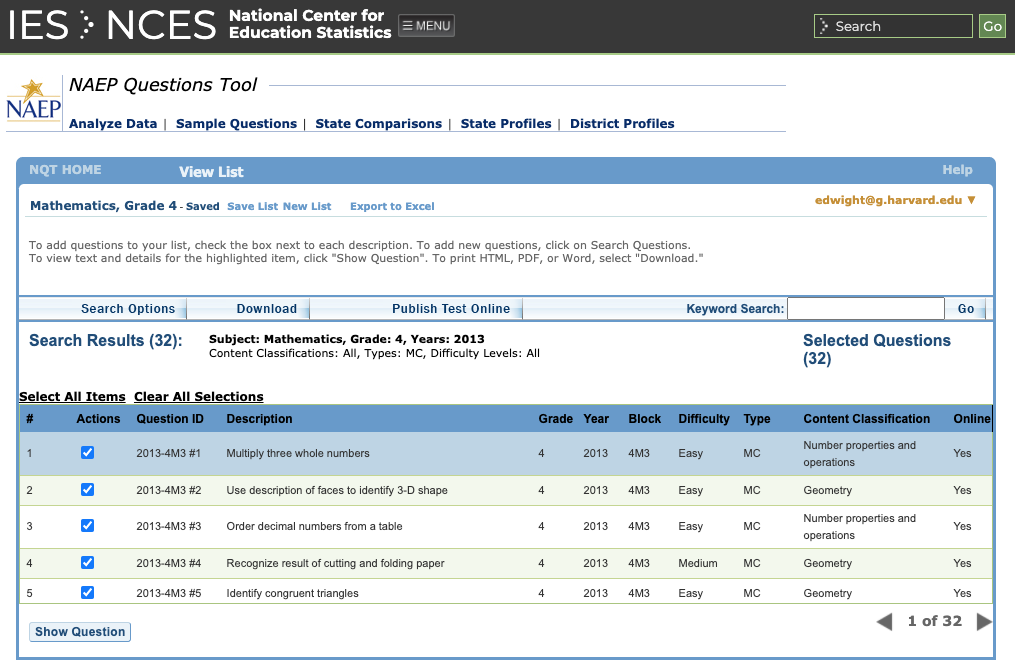
\includegraphics[width=0.7\linewidth]{images/1_released_items} 

}

\caption{https://nces.ed.gov/NationsReportCard/nqt/Search}\label{fig:unnamed-chunk-1}
\end{figure}

\begin{enumerate}
\def\labelenumi{\arabic{enumi})}
\setcounter{enumi}{1}
\tightlist
\item
  Released item IRT parameter estimates, like those found here: (Note
  that for NAEP, you will need to combine IRT parameters from each of
  the subscales to create an overall item pool)
\end{enumerate}

\textbackslash begin\{figure\}

\{\centering 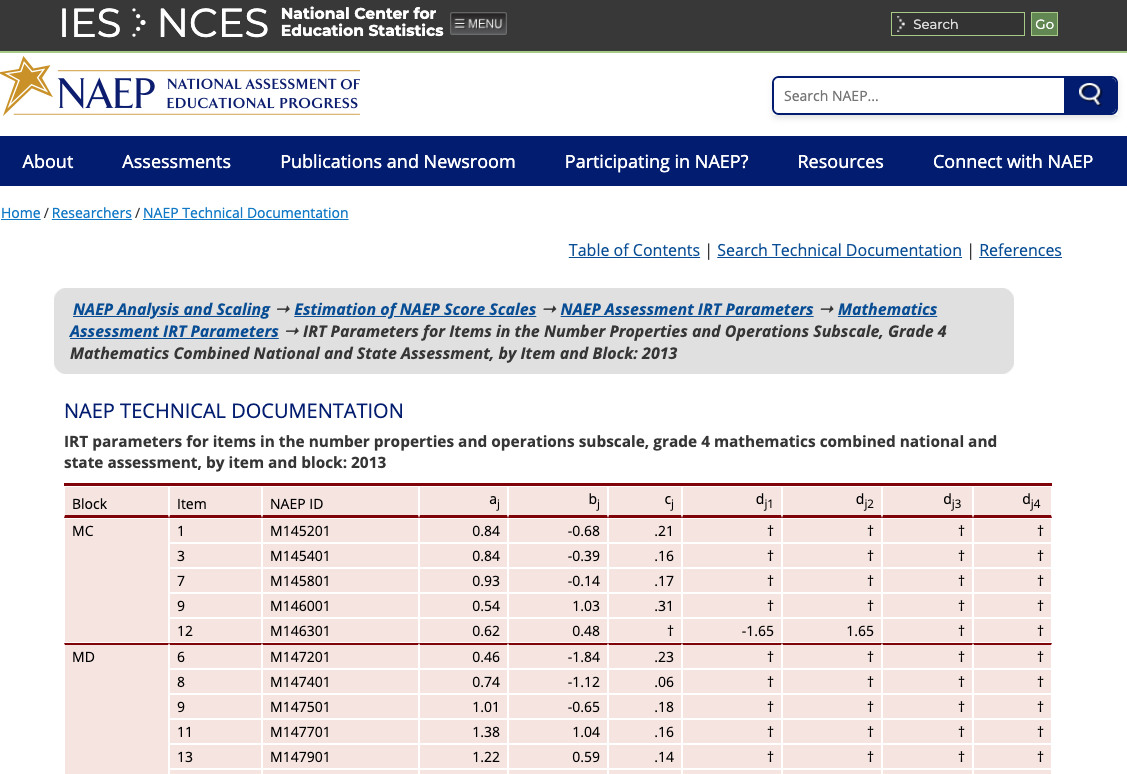
\includegraphics[width=0.7\linewidth]{images/2_item_parameters}

\}

\textbackslash caption\{\url{https://nces.ed.gov/nationsreportcard/tdw/analysis/scaling_irt_math.aspx\%7D/label\%7Bfig:unnamed-chunk-2}\}
\textbackslash end\{figure\}

\begin{enumerate}
\def\labelenumi{\arabic{enumi})}
\setcounter{enumi}{2}
\tightlist
\item
  Common item numbers/identifiers that relate each question (item) to
  its parameters: (To get the IDs for questions from NAEP, using the
  NAEP Questions Tool to select multiple choice questions from your
  chosen year, click OK, then select all items, then ``Export to
  Excel'')
\end{enumerate}

\begin{figure}

{\centering 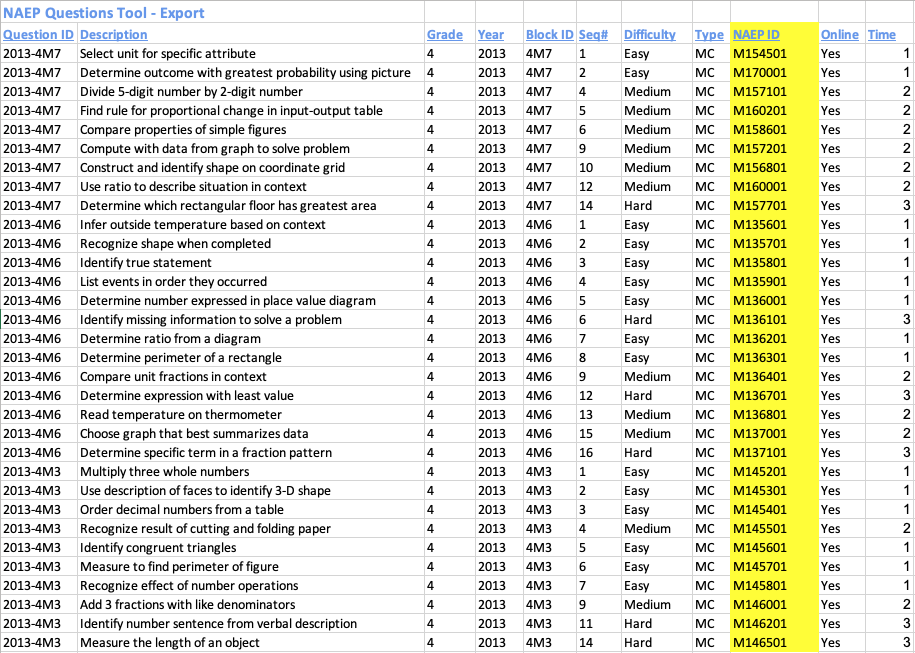
\includegraphics[width=0.7\linewidth]{images/3_questions_with_IDs} 

}

\caption{https://nces.ed.gov/NationsReportCard/nqt/Search#}\label{fig:unnamed-chunk-3}
\end{figure}

\begin{enumerate}
\def\labelenumi{\arabic{enumi})}
\setcounter{enumi}{3}
\item
  Student scores. For our tutorial, these can either be sum scores, or
  correct/incorrect responses for each of the test questions. (For NAEP
  items, you should consider exploring ``Download\ldots Test Kit'' for
  paper administration or ``Publish Test Online'' for online
  administration once you've chosen your items in the NAEP Questions
  Tool.)
\item
  An equation that converts theta scores to reporting scale scores (and
  possibly also achievement levels), like this:
\end{enumerate}

\textbackslash begin\{figure\}

\{\centering 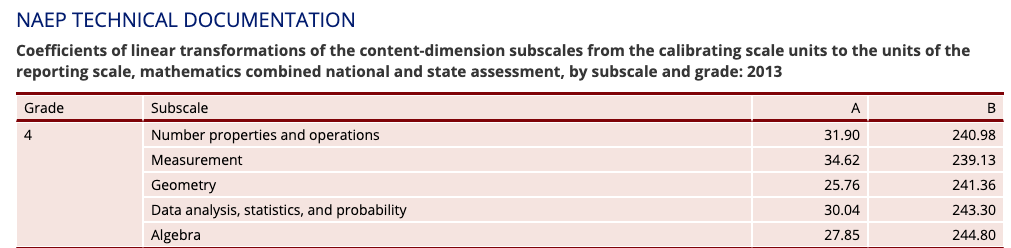
\includegraphics[width=0.7\linewidth]{images/5_theta_to_scale}

\}

\textbackslash caption\{\url{https://nces.ed.gov/nationsreportcard/tdw/analysis/trans_constants.aspx\%7D/label\%7Bfig:unnamed-chunk-4}\}
\textbackslash end\{figure\}

For NAEP, cut scores separating achievement level can be found here:
\url{https://nces.ed.gov/nationsreportcard/mathematics/achieve.asp\#grade4}

\hypertarget{contents}{%
\section{Contents:}\label{contents}}

\hypertarget{estimated-student-scale-scores-from-sum-scores}{%
\subsubsection{Estimated Student Scale Scores from Sum
Scores:}\label{estimated-student-scale-scores-from-sum-scores}}

\begin{itemize}
\tightlist
\item
  Import 3PL IRT item parameters
\item
  Import theta to scale score equation or table
\item
  Import (or simulate) student response data
\item
  Estimate student thetas using sum scores
\item
  Convert estimated thetas to scale scores
\item
  Produce table converting sum scores to scale scores, using Test
  Characteristic Curve information
\item
  Export student ability data, including estimated thetas, scale scores,
  and achievement levels
\end{itemize}

\hypertarget{appendix-1-simulating-imprecision-for-sum-score-theta-estimates}{%
\subsubsection{Appendix 1: Simulating Imprecision for Sum Score Theta
Estimates}\label{appendix-1-simulating-imprecision-for-sum-score-theta-estimates}}

\begin{itemize}
\tightlist
\item
  Invert the Test Characteristic Curve to Produce Estimates of Standard
  Errors
\item
  Produce table converting sum scores to scale scores, with empirical
  standard errors, using simulations
\end{itemize}

\hypertarget{appendix-2-scale-score-estimation-using-full-pattern-scoring}{%
\subsubsection{Appendix 2: Scale Score Estimation Using Full-Pattern
Scoring}\label{appendix-2-scale-score-estimation-using-full-pattern-scoring}}

\begin{itemize}
\tightlist
\item
  Estimate student ability using full-pattern scoring, (includes
  standard errors)
\item
  Export student ability data, including estimated thetas, standard
  errors, scale scores, and achievement levels
\end{itemize}

\hypertarget{appendix-3-diagnostics}{%
\subsubsection{Appendix 3: Diagnostics}\label{appendix-3-diagnostics}}

\begin{itemize}
\tightlist
\item
  Report Classical Test Theory statistics
\item
  Plot Item Characteristic Curves and Test Characteristic Curve
\item
  Plot Item Information Functions and Test Information Function
\end{itemize}

\hypertarget{appendix-4-replicating-naeps-theta-to-scale-score-equations}{%
\subsubsection{Appendix 4: Replicating NAEP's theta to scale score
equations}\label{appendix-4-replicating-naeps-theta-to-scale-score-equations}}

\begin{itemize}
\tightlist
\item
  Import table of theta to scale score equations (NAEP reports these
  separately by subscale)
\item
  Provide function to match NAEP's theta to scale score conversion,
  weighting transformation parameters appropriately
\end{itemize}

\hypertarget{appendix-5-creating-an-item-map-using-released-item-parameters}{%
\subsubsection{Appendix 5: Creating an item map, using released item
parameters}\label{appendix-5-creating-an-item-map-using-released-item-parameters}}

\begin{itemize}
\tightlist
\item
  Uses 3PL model to generate response probabilities for items
\item
  Creates table of item descriptions connected to scale scores for a
  chosen response probability
\end{itemize}

\hypertarget{estimated-student-scale-scores-from-sum-scores-1}{%
\section{Estimated Student Scale Scores from Sum
Scores:}\label{estimated-student-scale-scores-from-sum-scores-1}}

\hypertarget{importing-item-parameters-and-scale-scores}{%
\subsubsection{Importing item parameters and scale
scores}\label{importing-item-parameters-and-scale-scores}}

\begin{Shaded}
\begin{Highlighting}[]
\CommentTok{# Import selected items}
\NormalTok{selected_items <-}\StringTok{ }\KeywordTok{read.csv}\NormalTok{(}\StringTok{"Selected_Items.csv"}\NormalTok{, }\DataTypeTok{skip =} \DecValTok{1}\NormalTok{)}

\CommentTok{# Pull out vector of NAEP IDs for selected items}
\NormalTok{item_IDs <-}\StringTok{ }\NormalTok{selected_items}\OperatorTok{$}\NormalTok{NAEP.ID}

\CommentTok{# Import item parameter data}
\NormalTok{item_parameters_raw <-}\StringTok{ }\KeywordTok{read.csv}\NormalTok{(}\StringTok{"IRT_Parameters.csv"}\NormalTok{)                            }

\CommentTok{# Subset the item parameters, keeping only those whose IDs are in item_IDs}
\NormalTok{item_parameters_selected <-}\StringTok{ }\KeywordTok{subset}\NormalTok{(item_parameters_raw, item_parameters_raw}\OperatorTok{$}\NormalTok{NAEP.ID }\OperatorTok\StringTok{ }\NormalTok{item_IDs)}

\CommentTok{# Drop some unnecessary rows}
\NormalTok{item_parameters <-}\StringTok{ }\NormalTok{item_parameters_selected }\OperatorTok\StringTok{ }\NormalTok{dplyr}\OperatorTok{::}\KeywordTok{select}\NormalTok{(NAEP.ID, aj, bj, cj, Subscale)}

\CommentTok{# Turn this into the matrix form that irtoys expects}
\NormalTok{my_ip <-}\StringTok{ }\KeywordTok{as.matrix}\NormalTok{(item_parameters  }\OperatorTok\StringTok{ }\NormalTok{dplyr}\OperatorTok{::}\KeywordTok{select}\NormalTok{(aj, bj, cj))               }

\CommentTok{# NAEP Technical Documentation shows that a normalizing constant D of 1.7 is used in their 3PL equations:}
\CommentTok{# See here: https://nces.ed.gov/nationsreportcard/tdw/analysis/scaling_models_3pl.aspx}
\CommentTok{# The R package irtoys uses a normalizing constant of 1, so we adjust all NAEP parameters accordingly}
\NormalTok{D <-}\StringTok{ }\FloatTok{1.7}          \CommentTok{# Change to D = 1 if none appears in your technical report}
\CommentTok{# Divide "a" parameters by D to "undo" the normalizing constant and fit what the package irtoys expects}
\NormalTok{my_ip[,}\DecValTok{1}\NormalTok{] <-}\StringTok{ }\NormalTok{my_ip[,}\DecValTok{1}\NormalTok{]}\OperatorTok{/}\NormalTok{D}

\CommentTok{# View first five rows}
\NormalTok{my_ip[}\DecValTok{1}\OperatorTok{:}\DecValTok{5}\NormalTok{, ]}
\end{Highlighting}
\end{Shaded}

\begin{verbatim}
##           aj    bj   cj
## 1  0.4941176 -0.68 0.21
## 2  0.4941176 -0.39 0.16
## 3  0.5470588 -0.14 0.17
## 4  0.3176471  1.03 0.31
## 19 0.4411765 -0.62 0.39
\end{verbatim}

\begin{Shaded}
\begin{Highlighting}[]
\CommentTok{# Import student responses (if using real data)}


\CommentTok{# Takes theta(s), returns scale score(s) (for most tests, this looks like "scale_score = scale_multiplier*theta + scale_contant")}
\NormalTok{theta_to_scale_score <-}\StringTok{ }\ControlFlowTok{function}\NormalTok{(theta)}
\NormalTok{\{}
  \CommentTok{# NAEP uses a more complex weighted formula; we replicate that in Appendix 4}
  \CommentTok{# We simplify here by using the 2013 Grade 4 NAEP Math parameters for Number Properties and Operations, found here:}
  \CommentTok{# https://nces.ed.gov/nationsreportcard/tdw/analysis/2013/trans_constants_math2013.aspx}
\NormalTok{  scale_multiplier =}\StringTok{ }\FloatTok{31.90}
\NormalTok{  scale_constant =}\StringTok{ }\FloatTok{240.98}
  \KeywordTok{return}\NormalTok{(}\DataTypeTok{scale_score =}\NormalTok{ scale_multiplier}\OperatorTok{*}\NormalTok{theta }\OperatorTok{+}\StringTok{ }\NormalTok{scale_constant)}
\NormalTok{\}}


\CommentTok{# Takes theta(s), returns achievement levels}
\NormalTok{scale_score_to_achievement_level <-}\StringTok{ }\ControlFlowTok{function}\NormalTok{(scale_scores, }\DataTypeTok{cutoffs =} \KeywordTok{c}\NormalTok{(}\DecValTok{214}\NormalTok{, }\DecValTok{249}\NormalTok{, }\DecValTok{282}\NormalTok{))}
\NormalTok{\{}
  \CommentTok{# Note that these cutscores can vary by grade, subject, and year}
  \CommentTok{# Default cutoffs taken from here for 2013 grade 4 Math: }
  \CommentTok{# https://nces.ed.gov/nationsreportcard/mathematics/achieve.asp#grade4}
\NormalTok{  achievement_levels <-}\StringTok{ }\KeywordTok{rep}\NormalTok{(}\StringTok{"Below Basic"}\NormalTok{, }\KeywordTok{length}\NormalTok{(scale_scores)) }
\NormalTok{  achievement_levels[scale_scores }\OperatorTok{>=}\StringTok{ }\NormalTok{cutoffs[}\DecValTok{1}\NormalTok{]] <-}\StringTok{ "Basic"}
\NormalTok{  achievement_levels[scale_scores }\OperatorTok{>=}\StringTok{ }\NormalTok{cutoffs[}\DecValTok{2}\NormalTok{]] <-}\StringTok{ "Proficient"}
\NormalTok{  achievement_levels[scale_scores }\OperatorTok{>=}\StringTok{ }\NormalTok{cutoffs[}\DecValTok{3}\NormalTok{]] <-}\StringTok{ "Advanced"}
  \KeywordTok{return}\NormalTok{(achievement_levels)}
\NormalTok{\}}
\end{Highlighting}
\end{Shaded}

\hypertarget{scale-score-estimation-using-sum-scoring}{%
\subsubsection{Scale Score Estimation Using Sum
Scoring}\label{scale-score-estimation-using-sum-scoring}}

``Invert'' the TCC to get a map from sum scores to thetas:

\begin{Shaded}
\begin{Highlighting}[]
\CommentTok{# Plot Test Characteristic Curve (which underlies all of what follows)}
\CommentTok{# Theta on x axis, predicted sum score on y axis}
\KeywordTok{plot}\NormalTok{(}\KeywordTok{trf}\NormalTok{(my_ip))}
\end{Highlighting}
\end{Shaded}

\begin{center}\includegraphics{open-tests_files/figure-latex/unnamed-chunk-7-1} \end{center}

\begin{Shaded}
\begin{Highlighting}[]
\CommentTok{# Create a range of possible thetas}
\NormalTok{thetas =}\StringTok{ }\KeywordTok{seq}\NormalTok{(}\DataTypeTok{from =} \DecValTok{-5}\NormalTok{, }\DataTypeTok{to =} \DecValTok{5}\NormalTok{, }\DataTypeTok{length.out =} \DecValTok{100001}\NormalTok{)}
\CommentTok{# Calculate the estimated sum score for each of these thetas }
\NormalTok{all_sum_scores <-}\StringTok{ }\KeywordTok{trf}\NormalTok{(my_ip, }\DataTypeTok{x =}\NormalTok{ thetas)}

\CommentTok{# Simplifies the above possible sum scores (decimals) into possible whole number scores}
\NormalTok{possible_sum_scores <-}\StringTok{ }\KeywordTok{seq}\NormalTok{(}\DataTypeTok{from =} \KeywordTok{ceiling}\NormalTok{(all_sum_scores}\OperatorTok{$}\NormalTok{f[}\DecValTok{1}\NormalTok{]), }\DataTypeTok{to =} \KeywordTok{floor}\NormalTok{(all_sum_scores}\OperatorTok{$}\NormalTok{f[}\DecValTok{100000}\NormalTok{]), }\DataTypeTok{by =} \DecValTok{1}\NormalTok{)}

\CommentTok{# For each possible whole number score, find the associated theta that's the best match}
\NormalTok{matching_theta_scores <-}\StringTok{ }\KeywordTok{rep}\NormalTok{(}\OtherTok{NA}\NormalTok{, }\DataTypeTok{times =} \KeywordTok{length}\NormalTok{(possible_sum_scores))}
\ControlFlowTok{for}\NormalTok{(i }\ControlFlowTok{in} \DecValTok{1}\OperatorTok{:}\KeywordTok{length}\NormalTok{(possible_sum_scores)) \{matching_theta_scores[i] <-}\StringTok{ }\NormalTok{all_sum_scores}\OperatorTok{$}\NormalTok{x[}\KeywordTok{which.min}\NormalTok{(}\KeywordTok{abs}\NormalTok{(all_sum_scores}\OperatorTok{$}\NormalTok{f }\OperatorTok{-}\StringTok{ }\NormalTok{possible_sum_scores[i]))]\}}

\CommentTok{# Produce a table with sum scores, thetas, scale scores, and achievement levels}
\NormalTok{matching_theta_scores_df <-}\StringTok{ }\KeywordTok{as.data.frame}\NormalTok{(}\KeywordTok{cbind}\NormalTok{(possible_sum_scores, matching_theta_scores))}
\KeywordTok{colnames}\NormalTok{(matching_theta_scores_df) <-}\StringTok{ }\KeywordTok{c}\NormalTok{(}\StringTok{"SumScore"}\NormalTok{, }\StringTok{"Theta"}\NormalTok{)}

\CommentTok{# Convert the thetas to scale scores and then achievement levels, using our custom functions above}
\NormalTok{matching_theta_scores_df}\OperatorTok{$}\NormalTok{ScaleScore <-}\StringTok{ }\KeywordTok{theta_to_scale_score}\NormalTok{(matching_theta_scores_df}\OperatorTok{$}\NormalTok{Theta)}
\NormalTok{matching_theta_scores_df}\OperatorTok{$}\NormalTok{AchievementLevel <-}\StringTok{ }\KeywordTok{scale_score_to_achievement_level}\NormalTok{(matching_theta_scores_df}\OperatorTok{$}\NormalTok{ScaleScore)}

\CommentTok{# Round the Scale Scores before reporting}
\NormalTok{matching_theta_scores_df}\OperatorTok{$}\NormalTok{ScaleScore <-}\StringTok{ }\KeywordTok{round}\NormalTok{(matching_theta_scores_df}\OperatorTok{$}\NormalTok{ScaleScore)}

\CommentTok{# View table}
\NormalTok{matching_theta_scores_df}
\end{Highlighting}
\end{Shaded}

\begin{verbatim}
##    SumScore   Theta ScaleScore AchievementLevel
## 1         9 -4.3668        102      Below Basic
## 2        10 -3.5854        127      Below Basic
## 3        11 -2.9490        147      Below Basic
## 4        12 -2.4066        164      Below Basic
## 5        13 -1.9287        179      Below Basic
## 6        14 -1.4966        193      Below Basic
## 7        15 -1.0976        206      Below Basic
## 8        16 -0.7221        218            Basic
## 9        17 -0.3630        229            Basic
## 10       18 -0.0139        241            Basic
## 11       19  0.3305        252       Proficient
## 12       20  0.6756        263       Proficient
## 13       21  1.0269        274       Proficient
## 14       22  1.3905        285         Advanced
## 15       23  1.7737        298         Advanced
## 16       24  2.1861        311         Advanced
## 17       25  2.6412        325         Advanced
## 18       26  3.1596        342         Advanced
## 19       27  3.7756        361         Advanced
## 20       28  4.5549        386         Advanced
\end{verbatim}

\begin{Shaded}
\begin{Highlighting}[]
\CommentTok{# Export table}
\KeywordTok{write.csv}\NormalTok{(matching_theta_scores_df, }\DataTypeTok{file =} \StringTok{"Estimated_Scale_Scores_From_Sum_Scores.csv"}\NormalTok{, }\DataTypeTok{row.names =}\NormalTok{ F)}
\end{Highlighting}
\end{Shaded}

\hypertarget{appendix-1-simulating-imprecision-for-sum-score-theta-estimates-1}{%
\section{Appendix 1: Simulating Imprecision for Sum Score Theta
Estimates}\label{appendix-1-simulating-imprecision-for-sum-score-theta-estimates-1}}

How do we convey a sense of uncertainty with these sorts of score
estimates?

Because students with ``fixed'' thetas can retake the test and score
slightly differently each time, we simulate this below to create an
empirical range of possible scale scores for each student sum score.

\begin{Shaded}
\begin{Highlighting}[]
\CommentTok{# Create a sequence of possible thetas, equally spaced}
\NormalTok{sim_thetas <-}\StringTok{ }\KeywordTok{seq}\NormalTok{(}\DataTypeTok{from =} \DecValTok{-5}\NormalTok{, }\DataTypeTok{to =} \DecValTok{5}\NormalTok{, }\DataTypeTok{length.out =} \DecValTok{1001}\NormalTok{)}

\CommentTok{# Replicate each of the possible thetas 100 times, as if each of these students took the test 100 times}
\NormalTok{sim_thetas_n <-}\StringTok{ }\KeywordTok{rep}\NormalTok{(sim_thetas, }\DataTypeTok{each =} \DecValTok{100}\NormalTok{)}

\CommentTok{# Simulate the sum scores that these students received, using the item parameters for this test (assume these item parameters are estimated perfectly)}
\NormalTok{sim_sum_scores <-}\StringTok{ }\KeywordTok{rowSums}\NormalTok{(}\KeywordTok{sim}\NormalTok{(my_ip, sim_thetas_n))}

\CommentTok{# Combine the thetas and sum scores into a data frame}
\NormalTok{sim1_long <-}\StringTok{ }\KeywordTok{as.data.frame}\NormalTok{(}\KeywordTok{cbind}\NormalTok{(sim_thetas_n, sim_sum_scores))}

\CommentTok{# Rename column to the name expected by theta_to_scale_score conversion}
\KeywordTok{colnames}\NormalTok{(sim1_long) <-}\StringTok{ }\KeywordTok{c}\NormalTok{(}\StringTok{"Theta"}\NormalTok{, }\StringTok{"sim_sum_scores"}\NormalTok{)}

\CommentTok{# Add column for scale scores (from thetas)}
\NormalTok{sim1_long}\OperatorTok{$}\NormalTok{sim_scale_scores <-}\StringTok{ }\KeywordTok{theta_to_scale_score}\NormalTok{(sim1_long}\OperatorTok{$}\NormalTok{Theta)}

\CommentTok{# Group the above data frame by sum scores, and summarize the different "true" thetas that could have produced each sum score}
\NormalTok{sim1_thetas <-}\StringTok{ }\NormalTok{sim1_long }\OperatorTok\StringTok{ }
\StringTok{  }\KeywordTok{group_by}\NormalTok{(sim_sum_scores) }\OperatorTok\StringTok{ }
\StringTok{  }\KeywordTok{summarise}\NormalTok{(}\KeywordTok{tibble}\NormalTok{(}\StringTok{'2.5'}\NormalTok{ =}\StringTok{ }\KeywordTok{round}\NormalTok{(}\KeywordTok{quantile}\NormalTok{(sim_scale_scores, }\FloatTok{0.025}\NormalTok{), }\DecValTok{0}\NormalTok{),}
                   \StringTok{'10'}\NormalTok{ =}\StringTok{ }\KeywordTok{round}\NormalTok{(}\KeywordTok{quantile}\NormalTok{(sim_scale_scores, }\FloatTok{0.1}\NormalTok{), }\DecValTok{0}\NormalTok{),}
                   \DataTypeTok{mean =} \KeywordTok{round}\NormalTok{(}\KeywordTok{mean}\NormalTok{(sim_scale_scores), }\DecValTok{0}\NormalTok{), }
                   \DataTypeTok{median =} \KeywordTok{round}\NormalTok{(}\KeywordTok{median}\NormalTok{(sim_scale_scores), }\DecValTok{0}\NormalTok{), }
                   \DataTypeTok{se =} \KeywordTok{round}\NormalTok{(}\KeywordTok{sd}\NormalTok{(sim_scale_scores), }\DecValTok{1}\NormalTok{),}
                   \StringTok{'90'}\NormalTok{ =}\StringTok{ }\KeywordTok{round}\NormalTok{(}\KeywordTok{quantile}\NormalTok{(sim_scale_scores, }\FloatTok{0.9}\NormalTok{), }\DecValTok{0}\NormalTok{),}
                   \StringTok{'97.5'}\NormalTok{ =}\StringTok{ }\KeywordTok{round}\NormalTok{(}\KeywordTok{quantile}\NormalTok{(sim_scale_scores, }\FloatTok{0.975}\NormalTok{), }\DecValTok{0}\NormalTok{), }
                   \DataTypeTok{max =} \KeywordTok{round}\NormalTok{(}\KeywordTok{max}\NormalTok{(sim_scale_scores), }\DecValTok{0}\NormalTok{),}
                   \DataTypeTok{nsims =} \KeywordTok{n}\NormalTok{()))}
\NormalTok{sim1_thetas}
\end{Highlighting}
\end{Shaded}

\begin{verbatim}
## # A tibble: 31 x 10
##    sim_sum_scores `2.5`  `10`  mean median    se  `90` `97.5`   max nsims
##             <dbl> <dbl> <dbl> <dbl>  <dbl> <dbl> <dbl>  <dbl> <dbl> <int>
##  1              1    88    88   102     96  15.7   122    122   122     6
##  2              2    85    87   105     99  18.9   132    146   148    28
##  3              3    82    84   101     97  16.5   122    143   158    94
##  4              4    83    85   104     98  17.7   129    147   161   339
##  5              5    82    86   110    104  22.2   142    162   207   756
##  6              6    82    86   112    106  24.2   147    170   211  1491
##  7              7    83    87   116    111  25.7   153    175   220  2441
##  8              8    83    88   122    117  28.2   161    185   229  3355
##  9              9    83    90   129    124  31.4   173    196   252  4243
## 10             10    84    93   136    133  33.6   183    206   256  4731
## # ... with 21 more rows
\end{verbatim}

\begin{Shaded}
\begin{Highlighting}[]
\CommentTok{# Repeat the above, this time summarizing the different "true" scale scores that could have produced each sum score}
\NormalTok{sim1_scale_scores <-}\StringTok{ }\NormalTok{sim1_long }\OperatorTok\StringTok{ }
\StringTok{  }\KeywordTok{group_by}\NormalTok{(sim_sum_scores) }\OperatorTok\StringTok{ }
\StringTok{  }\KeywordTok{summarise}\NormalTok{(}\KeywordTok{tibble}\NormalTok{(}\StringTok{'2.5'}\NormalTok{ =}\StringTok{ }\KeywordTok{round}\NormalTok{(}\KeywordTok{quantile}\NormalTok{(sim_scale_scores, }\FloatTok{0.025}\NormalTok{), }\DecValTok{0}\NormalTok{),}
                   \StringTok{'10'}\NormalTok{ =}\StringTok{ }\KeywordTok{round}\NormalTok{(}\KeywordTok{quantile}\NormalTok{(sim_scale_scores, }\FloatTok{0.1}\NormalTok{), }\DecValTok{0}\NormalTok{),}
                   \DataTypeTok{mean =} \KeywordTok{round}\NormalTok{(}\KeywordTok{mean}\NormalTok{(sim_scale_scores), }\DecValTok{0}\NormalTok{), }
                   \DataTypeTok{median =} \KeywordTok{round}\NormalTok{(}\KeywordTok{median}\NormalTok{(sim_scale_scores), }\DecValTok{0}\NormalTok{), }
                   \DataTypeTok{se =} \KeywordTok{round}\NormalTok{(}\KeywordTok{sd}\NormalTok{(sim_scale_scores), }\DecValTok{1}\NormalTok{),}
                   \StringTok{'90'}\NormalTok{ =}\StringTok{ }\KeywordTok{round}\NormalTok{(}\KeywordTok{quantile}\NormalTok{(sim_scale_scores, }\FloatTok{0.9}\NormalTok{), }\DecValTok{0}\NormalTok{),}
                   \StringTok{'97.5'}\NormalTok{ =}\StringTok{ }\KeywordTok{round}\NormalTok{(}\KeywordTok{quantile}\NormalTok{(sim_scale_scores, }\FloatTok{0.975}\NormalTok{), }\DecValTok{0}\NormalTok{), }
                   \DataTypeTok{max =} \KeywordTok{round}\NormalTok{(}\KeywordTok{max}\NormalTok{(sim_scale_scores), }\DecValTok{0}\NormalTok{),}
                   \DataTypeTok{nsims =} \KeywordTok{n}\NormalTok{()))}
\NormalTok{sim1_scale_scores}
\end{Highlighting}
\end{Shaded}

\begin{verbatim}
## # A tibble: 31 x 10
##    sim_sum_scores `2.5`  `10`  mean median    se  `90` `97.5`   max nsims
##             <dbl> <dbl> <dbl> <dbl>  <dbl> <dbl> <dbl>  <dbl> <dbl> <int>
##  1              1    88    88   102     96  15.7   122    122   122     6
##  2              2    85    87   105     99  18.9   132    146   148    28
##  3              3    82    84   101     97  16.5   122    143   158    94
##  4              4    83    85   104     98  17.7   129    147   161   339
##  5              5    82    86   110    104  22.2   142    162   207   756
##  6              6    82    86   112    106  24.2   147    170   211  1491
##  7              7    83    87   116    111  25.7   153    175   220  2441
##  8              8    83    88   122    117  28.2   161    185   229  3355
##  9              9    83    90   129    124  31.4   173    196   252  4243
## 10             10    84    93   136    133  33.6   183    206   256  4731
## # ... with 21 more rows
\end{verbatim}

\begin{Shaded}
\begin{Highlighting}[]
\CommentTok{# Can also create a histogram for the possible thetas that produced each sum score, for example:}
\KeywordTok{hist}\NormalTok{(sim1_long}\OperatorTok{$}\NormalTok{Theta[sim1_long}\OperatorTok{$}\NormalTok{sim_sum_scores }\OperatorTok{==}\StringTok{ }\DecValTok{20}\NormalTok{], }\DataTypeTok{freq =}\NormalTok{ F)}
\end{Highlighting}
\end{Shaded}

\begin{center}\includegraphics{open-tests_files/figure-latex/unnamed-chunk-8-1} \end{center}

\hypertarget{appendix-2-scale-score-estimation-using-full-pattern-scoring-1}{%
\section{Appendix 2: Scale Score Estimation Using Full-Pattern
Scoring}\label{appendix-2-scale-score-estimation-using-full-pattern-scoring-1}}

Full-pattern scoring (using a full table recording how each student
performed on each question) can improve ability estimation.

\begin{Shaded}
\begin{Highlighting}[]
\CommentTok{# Use parameter estimates to simulate answers for 100 students}
\CommentTok{# (Import student data here if using real answers)}
\KeywordTok{set.seed}\NormalTok{(}\DecValTok{88}\NormalTok{)}
\NormalTok{sim_thetas <-}\StringTok{ }\KeywordTok{rnorm}\NormalTok{(}\DecValTok{1000}\NormalTok{)}
\NormalTok{sim_responses <-}\StringTok{ }\KeywordTok{sim}\NormalTok{(my_ip, sim_thetas)}

\CommentTok{# Put the parameter estimates and standard errors into the list structure that irtoys functions expect}
\CommentTok{# Note: ability estimation function does not need standard errors or variance-covariance matrix to run}
\NormalTok{parameter_list <-}\StringTok{ }\KeywordTok{list}\NormalTok{(}\DataTypeTok{est =}\NormalTok{ my_ip, }\DataTypeTok{se =} \OtherTok{NA}\NormalTok{, }\DataTypeTok{vcm =} \OtherTok{NA}\NormalTok{)}

\CommentTok{# Estimate student thetas, based on full-pattern scoring, using MLE (several other methods exist for this "ability" function)}
\NormalTok{mod_MLE<-}\StringTok{ }\KeywordTok{ability}\NormalTok{(}\DataTypeTok{resp =}\NormalTok{ sim_responses, }\DataTypeTok{ip =}\NormalTok{ parameter_list, }\DataTypeTok{method =} \StringTok{"MLE"}\NormalTok{)}

\CommentTok{# Look at the first five rows}
\NormalTok{mod_MLE[}\DecValTok{1}\OperatorTok{:}\DecValTok{5}\NormalTok{, ]}
\end{Highlighting}
\end{Shaded}

\begin{verbatim}
##             est       sem  n
## [1,] -1.1985497 1.0216098 31
## [2,]  0.4882736 0.8668540 31
## [3,]  2.9747950 1.0424542 31
## [4,] -2.1205461 1.2139283 31
## [5,]  0.5835620 0.8651891 31
\end{verbatim}

\begin{Shaded}
\begin{Highlighting}[]
\CommentTok{# Convert these estimated thetas to scale scores and achievement levels}
\NormalTok{ability_df <-}\StringTok{ }\KeywordTok{as.data.frame}\NormalTok{(mod_MLE)}
\KeywordTok{colnames}\NormalTok{(ability_df) <-}\StringTok{ }\KeywordTok{c}\NormalTok{(}\StringTok{"Theta"}\NormalTok{, }\StringTok{"se(Theta)"}\NormalTok{, }\StringTok{"QuestionsAnswered"}\NormalTok{)}
\NormalTok{ability_df}\OperatorTok{$}\NormalTok{ScaleScore <-}\StringTok{ }\KeywordTok{theta_to_scale_score}\NormalTok{(ability_df}\OperatorTok{$}\NormalTok{Theta)}
\NormalTok{ability_df}\OperatorTok{$}\NormalTok{AchievementLevel <-}\StringTok{ }\KeywordTok{scale_score_to_achievement_level}\NormalTok{(ability_df}\OperatorTok{$}\NormalTok{ScaleScore)}

\CommentTok{# Round the scale scores to 0 dp before reporting}
\NormalTok{ability_df}\OperatorTok{$}\NormalTok{ScaleScore <-}\StringTok{ }\KeywordTok{round}\NormalTok{(ability_df}\OperatorTok{$}\NormalTok{ScaleScore, }\DecValTok{0}\NormalTok{)}

\CommentTok{# View table:}
\NormalTok{ability_df}
\end{Highlighting}
\end{Shaded}

\begin{verbatim}
##             Theta se(Theta) QuestionsAnswered ScaleScore AchievementLevel
## 1    -1.198549721 1.0216098                31        203      Below Basic
## 2     0.488273592 0.8668540                31        257       Proficient
## 3     2.974794957 1.0424542                31        336         Advanced
## 4    -2.120546071 1.2139283                31        173      Below Basic
## 5     0.583561985 0.8651891                31        260       Proficient
## 6     0.345894269 0.8706878                31        252       Proficient
## 7    -0.233786359 0.9033941                31        234            Basic
## 8    -3.999931695 1.8805408                31        113      Below Basic
## 9    -1.365085407 1.0504287                31        197      Below Basic
## 10    0.239805324 0.8746052                31        249            Basic
## 11   -1.578158011 1.0910399                31        191      Below Basic
## 12    2.346990431 0.9567203                31        316         Advanced
## 13    1.808157751 0.9050213                31        299         Advanced
## 14   -0.753307669 0.9568772                31        217            Basic
## 15    0.791131314 0.8640252                31        266       Proficient
## 16   -0.196600598 0.9004549                31        235            Basic
## 17    1.635665341 0.8927793                31        293         Advanced
## 18    1.697093620 0.8968969                31        295         Advanced
## 19   -1.082020734 1.0029485                31        206      Below Basic
## 20    1.896567224 0.9121108                31        301         Advanced
## 21   -0.739271530 0.9551235                31        217            Basic
## 22   -1.365710222 1.0505416                31        197      Below Basic
## 23    0.349945854 0.8705562                31        252       Proficient
## 24   -1.466929427 1.0693121                31        194      Below Basic
## 25    0.424275451 0.8683766                31        255       Proficient
## 26   -1.241706366 1.0288342                31        201      Below Basic
## 27    0.418267288 0.8685364                31        254       Proficient
## 28   -0.521145456 0.9300892                31        224            Basic
## 29   -1.910636828 1.1629829                31        180      Below Basic
## 30   -0.999830571 0.9905239                31        209      Below Basic
## 31   -0.737928454 0.9549566                31        217            Basic
## 32    1.536023877 0.8866726                31        290         Advanced
## 33    1.031615325 0.8668194                31        274       Proficient
## 34    0.009679705 0.8862644                31        241            Basic
## 35    0.729741815 0.8640208                31        264       Proficient
## 36   -1.757093352 1.1284430                31        185      Below Basic
## 37   -2.077234742 1.2030598                31        175      Below Basic
## 38    0.657791258 0.8643874                31        262       Proficient
## 39   -2.412642286 1.2921690                31        164      Below Basic
## 40   -3.999925722 1.8805380                31        113      Below Basic
## 41    1.581776574 0.8893884                31        291         Advanced
## 42    1.564930928 0.8883711                31        291         Advanced
## 43   -0.208184722 0.9013580                31        234            Basic
## 44    0.606297565 0.8648976                31        260       Proficient
## 45   -2.687903925 1.3739830                31        155      Below Basic
## 46   -0.666917534 0.9463583                31        220            Basic
## 47   -0.725564890 0.9534278                31        218            Basic
## 48    1.967282610 0.9181769                31        304         Advanced
## 49    0.488729700 0.8668443                31        257       Proficient
## 50    0.327556184 0.8712999                31        251       Proficient
## 51    0.474317476 0.8671582                31        256       Proficient
## 52    0.374732686 0.8697801                31        253       Proficient
## 53   -3.016774649 1.4824131                31        145      Below Basic
## 54    0.734725073 0.8640103                31        264       Proficient
## 55   -0.124560024 0.8950931                31        237            Basic
## 56    0.822850498 0.8641413                31        267       Proficient
## 57   -0.312478771 0.9100014                31        231            Basic
## 58   -0.124743925 0.8951063                31        237            Basic
## 59    1.797907912 0.9042350                31        298         Advanced
## 60    0.224607093 0.8752412                31        248            Basic
## 61    1.174171120 0.8705329                31        278       Proficient
## 62   -0.283438754 0.9075017                31        232            Basic
## 63    1.292419862 0.8747559                31        282         Advanced
## 64    1.655656636 0.8940898                31        294         Advanced
## 65   -0.268751769 0.9062649                31        232            Basic
## 66   -0.785942114 0.9610217                31        216            Basic
## 67    0.812599053 0.8640954                31        267       Proficient
## 68    0.659754614 0.8643720                31        262       Proficient
## 69    1.823755771 0.9062321                31        299         Advanced
## 70   -1.506668114 1.0769419                31        193      Below Basic
## 71    0.983480115 0.8659091                31        272       Proficient
## 72   -1.021834756 0.9937907                31        208      Below Basic
## 73    2.632222033 0.9922681                31        325         Advanced
## 74    1.505788331 0.8849603                31        289         Advanced
## 75   -0.186092220 0.8996455                31        235            Basic
## 76    2.209784147 0.9416342                31        311         Advanced
## 77    1.753047876 0.9008809                31        297         Advanced
## 78   -0.990964271 0.9892199                31        209      Below Basic
## 79    1.204315917 0.8715116                31        279       Proficient
## 80   -1.091020918 1.0043460                31        206      Below Basic
## 81    0.585329734 0.8651650                31        260       Proficient
## 82   -0.561673185 0.9344267                31        223            Basic
## 83    0.295791145 0.8724243                31        250       Proficient
## 84    0.426973383 0.8683058                31        255       Proficient
## 85   -1.227447014 1.0264284                31        202      Below Basic
## 86    0.119843845 0.8801392                31        245            Basic
## 87   -0.964978640 0.9854385                31        210      Below Basic
## 88   -1.777910298 1.1329926                31        184      Below Basic
## 89   -0.487507015 0.9265972                31        225            Basic
## 90   -0.229692969 0.9030648                31        234            Basic
## 91   -0.892341259 0.9751887                31        213      Below Basic
## 92    0.499837338 0.8666136                31        257       Proficient
## 93   -1.435484433 1.0633790                31        195      Below Basic
## 94   -1.662936714 1.1083824                31        188      Below Basic
## 95    2.630054605 0.9919767                31        325         Advanced
## 96   -0.199367278 0.9006695                31        235            Basic
## 97    1.584278948 0.8895413                31        292         Advanced
## 98    0.550081429 0.8656923                31        259       Proficient
## 99    1.330889612 0.8763511                31        283         Advanced
## 100  -0.476205433 0.9254460                31        226            Basic
## 101  -0.176585984 0.8989213                31        235            Basic
## 102  -1.886097662 1.1573095                31        181      Below Basic
## 103  -2.599175041 1.3467367                31        158      Below Basic
## 104  -3.999928759 1.8805394                31        113      Below Basic
## 105  -0.744939668 0.9558296                31        217            Basic
## 106   1.305829992 0.8752997                31        283         Advanced
## 107  -2.328535698 1.2687486                31        167      Below Basic
## 108  -0.498930657 0.9277721                31        225            Basic
## 109  -1.711264866 1.1185733                31        186      Below Basic
## 110   1.274755891 0.8740598                31        282       Proficient
## 111   0.040564924 0.8844458                31        242            Basic
## 112  -0.388167886 0.9168551                31        229            Basic
## 113   0.756664924 0.8639869                31        265       Proficient
## 114   0.668313777 0.8643086                31        262       Proficient
## 115   2.187485846 0.9393062                31        311         Advanced
## 116  -0.697558009 0.9500141                31        219            Basic
## 117   0.154434963 0.8784225                31        246            Basic
## 118   1.472923456 0.8831737                31        288         Advanced
## 119   1.212852422 0.8718009                31        280       Proficient
## 120   1.998976724 0.9210094                31        305         Advanced
## 121   1.051679427 0.8672503                31        275       Proficient
## 122   1.231130786 0.8724385                31        280       Proficient
## 123   0.161397558 0.8780888                31        246            Basic
## 124  -0.302465646 0.9091314                31        231            Basic
## 125   0.144296306 0.8789154                31        246            Basic
## 126   0.065933064 0.8830112                31        243            Basic
## 127   0.129185001 0.8796659                31        245            Basic
## 128  -0.025072637 0.8884056                31        240            Basic
## 129   2.102307760 0.9307318                31        308         Advanced
## 130   0.619096584 0.8647514                31        261       Proficient
## 131  -2.860348737 1.4293609                31        150      Below Basic
## 132  -2.220500408 1.2397274                31        170      Below Basic
## 133  -0.782206467 0.9605426                31        216            Basic
## 134  -1.135570301 1.0113712                31        205      Below Basic
## 135  -0.973763755 0.9867101                31        210      Below Basic
## 136   0.319968447 0.8715610                31        251       Proficient
## 137   2.568464952 0.9838315                31        323         Advanced
## 138  -1.649609542 1.1056111                31        188      Below Basic
## 139  -2.392596541 1.2865208                31        165      Below Basic
## 140   0.468938574 0.8672796                31        256       Proficient
## 141  -3.999955515 1.8805519                31        113      Below Basic
## 142   0.033372527 0.8848622                31        242            Basic
## 143  -0.945288257 0.9826135                31        211      Below Basic
## 144   2.013800911 0.9223584                31        305         Advanced
## 145  -0.573816925 0.9357541                31        223            Basic
## 146   0.153629881 0.8784613                31        246            Basic
## 147   0.355654193 0.8703731                31        252       Proficient
## 148  -1.266377218 1.0330405                31        201      Below Basic
## 149  -1.939436358 1.1697161                31        179      Below Basic
## 150  -0.959749859 0.9846850                31        210      Below Basic
## 151   1.900673861 0.9124535                31        302         Advanced
## 152  -0.234196055 0.9034272                31        234            Basic
## 153  -0.206285356 0.9012091                31        234            Basic
## 154  -1.922398020 1.1657228                31        180      Below Basic
## 155   0.040951885 0.8844235                31        242            Basic
## 156   0.073127672 0.8826141                31        243            Basic
## 157   1.188522016 0.8709904                31        279       Proficient
## 158   2.011175143 0.9221183                31        305         Advanced
## 159  -2.215669915 1.2384575                31        170      Below Basic
## 160   0.736933684 0.8640063                31        264       Proficient
## 161  -0.724782921 0.9533315                31        218            Basic
## 162  -1.389668035 1.0548987                31        197      Below Basic
## 163  -0.456287469 0.9234439                31        226            Basic
## 164   0.713504004 0.8640684                31        264       Proficient
## 165  -1.363213703 1.0500906                31        197      Below Basic
## 166  -0.310689856 0.9098453                31        231            Basic
## 167   1.800545684 0.9044366                31        298         Advanced
## 168   1.788301474 0.9035047                31        298         Advanced
## 169  -0.758370434 0.9575140                31        217            Basic
## 170  -0.228571100 0.9029748                31        234            Basic
## 171   2.745467575 1.0079511                31        329         Advanced
## 172  -2.584220330 1.3422270                31        159      Below Basic
## 173   0.999510659 0.8661928                31        273       Proficient
## 174   2.186752256 0.9392301                31        311         Advanced
## 175   0.389694374 0.8693355                31        253       Proficient
## 176  -1.518151645 1.0791742                31        193      Below Basic
## 177  -1.118838758 1.0087117                31        205      Below Basic
## 178  -1.717711403 1.1199495                31        186      Below Basic
## 179  -2.548309901 1.3314945                31        160      Below Basic
## 180   1.627746200 0.8922680                31        293         Advanced
## 181  -0.185314658 0.8995860                31        235            Basic
## 182   1.157045568 0.8700068                31        278       Proficient
## 183   0.873698204 0.8644883                31        269       Proficient
## 184   0.136930100 0.8792789                31        245            Basic
## 185   0.096812517 0.8813368                31        244            Basic
## 186  -0.123314706 0.8950043                31        237            Basic
## 187  -1.327407840 1.0436858                31        199      Below Basic
## 188   1.964363907 0.9179196                31        304         Advanced
## 189   0.250365164 0.8741744                31        249            Basic
## 190  -0.005375007 0.8871796                31        241            Basic
## 191  -0.205921955 0.9011807                31        234            Basic
## 192   0.219617268 0.8754542                31        248            Basic
## 193  -1.230100270 1.0268746                31        202      Below Basic
## 194  -1.327756949 1.0437476                31        199      Below Basic
## 195  -0.046093109 0.8897496                31        240            Basic
## 196   1.086572470 0.8680714                31        276       Proficient
## 197  -1.015877747 0.9929020                31        209      Below Basic
## 198  -0.433106179 0.9211569                31        227            Basic
## 199   0.209863303 0.8758762                31        248            Basic
## 200  -0.066975088 0.8911213                31        239            Basic
## 201   1.049022705 0.8671915                31        274       Proficient
## 202  -3.789593524 1.7856504                31        120      Below Basic
## 203   1.156877097 0.8700017                31        278       Proficient
## 204   1.610705997 0.8911830                31        292         Advanced
## 205   1.352696255 0.8773034                31        284         Advanced
## 206   0.075662911 0.8824751                31        243            Basic
## 207  -0.067088269 0.8911288                31        239            Basic
## 208   2.916885366 1.0333937                31        334         Advanced
## 209   0.592945168 0.8650639                31        260       Proficient
## 210   1.520417152 0.8857806                31        289         Advanced
## 211  -0.212314113 0.9016826                31        234            Basic
## 212   0.630434809 0.8646326                31        261       Proficient
## 213  -1.481772721 1.0721448                31        194      Below Basic
## 214   0.969969644 0.8656849                31        272       Proficient
## 215  -2.151330872 1.2217673                31        172      Below Basic
## 216  -1.426789937 1.0617548                31        195      Below Basic
## 217  -2.001278081 1.1844488                31        177      Below Basic
## 218  -1.175850502 1.0178780                31        203      Below Basic
## 219   1.716780292 0.8982733                31        296         Advanced
## 220  -3.088498255 1.5076499                31        142      Below Basic
## 221   0.990406147 0.8660293                31        273       Proficient
## 222   0.903129275 0.8647794                31        270       Proficient
## 223  -0.104865120 0.8937034                31        238            Basic
## 224  -3.040690822 1.4907641                31        144      Below Basic
## 225   0.293894392 0.8724940                31        250       Proficient
## 226   0.912892808 0.8648905                31        270       Proficient
## 227  -1.753107857 1.1275767                31        185      Below Basic
## 228   0.099281610 0.8812063                31        244            Basic
## 229  -3.999927932 1.8805391                31        113      Below Basic
## 230   0.324491614 0.8714048                31        251       Proficient
## 231  -0.179228327 0.8991219                31        235            Basic
## 232   0.157627648 0.8782690                31        246            Basic
## 233  -0.356637581 0.9139404                31        230            Basic
## 234   0.052170367 0.8837829                31        243            Basic
## 235   0.735446123 0.8640090                31        264       Proficient
## 236  -0.437161062 0.9215536                31        227            Basic
## 237   0.129955916 0.8796271                31        245            Basic
## 238  -0.908120764 0.9773753                31        212      Below Basic
## 239   0.894178173 0.8646839                31        270       Proficient
## 240   0.576447708 0.8652886                31        259       Proficient
## 241   2.063187878 0.9269633                31        307         Advanced
## 242   0.179256519 0.8772511                31        247            Basic
## 243  -0.758104798 0.9574806                31        217            Basic
## 244   0.264750993 0.8736020                31        249       Proficient
## 245   1.703214554 0.8973219                31        295         Advanced
## 246   0.777833119 0.8639996                31        266       Proficient
## 247  -0.435028784 0.9213448                31        227            Basic
## 248  -1.801450003 1.1381874                31        184      Below Basic
## 249  -0.239720680 0.9038740                31        233            Basic
## 250   3.327631025 1.1027768                31        347         Advanced
## 251   0.528412196 0.8660652                31        258       Proficient
## 252  -0.473918267 0.9252143                31        226            Basic
## 253  -0.312228094 0.9099795                31        231            Basic
## 254  -1.119777207 1.0088602                31        205      Below Basic
## 255  -1.297586818 1.0384415                31        200      Below Basic
## 256   0.905341688 0.8648039                31        270       Proficient
## 257   0.211914657 0.8757868                31        248            Basic
## 258  -0.772630675 0.9593199                31        216            Basic
## 259  -1.433047223 1.0629230                31        195      Below Basic
## 260   0.731268905 0.8640174                31        264       Proficient
## 261   0.176805190 0.8773646                31        247            Basic
## 262   0.026760998 0.8852488                31        242            Basic
## 263   1.098346584 0.8683690                31        276       Proficient
## 264  -1.476127896 1.0710651                31        194      Below Basic
## 265  -0.414206461 0.9193265                31        228            Basic
## 266  -0.412093330 0.9191238                31        228            Basic
## 267   0.789334520 0.8640210                31        266       Proficient
## 268   0.114522519 0.8804120                31        245            Basic
## 269  -0.205219359 0.9011257                31        234            Basic
## 270   0.224542529 0.8752440                31        248            Basic
## 271   1.448837164 0.8819138                31        287         Advanced
## 272  -2.633779369 1.3572629                31        157      Below Basic
## 273  -0.573130466 0.9356788                31        223            Basic
## 274   3.999922841 1.2425602                31        369         Advanced
## 275   0.311310707 0.8718647                31        251       Proficient
## 276  -1.020015273 0.9935189                31        208      Below Basic
## 277  -0.026720239 0.8885096                31        240            Basic
## 278  -2.354045695 1.2757752                31        166      Below Basic
## 279  -2.045299850 1.1951656                31        176      Below Basic
## 280   2.447267146 0.9685732                31        319         Advanced
## 281  -3.207571961 1.5508310                31        139      Below Basic
## 282  -1.319162121 1.0422275                31        199      Below Basic
## 283   1.950602413 0.9167145                31        303         Advanced
## 284   3.201529429 1.0802035                31        343         Advanced
## 285   2.650553764 0.9947462                31        326         Advanced
## 286  -0.114031901 0.8943462                31        237            Basic
## 287  -0.927613719 0.9801072                31        211      Below Basic
## 288  -1.023077170 0.9939764                31        208      Below Basic
## 289   1.524912375 0.8860357                31        290         Advanced
## 290   1.252174392 0.8732031                31        281       Proficient
## 291   1.604617607 0.8908003                31        292         Advanced
## 292  -1.526465034 1.0807979                31        192      Below Basic
## 293   1.802494936 0.9045859                31        298         Advanced
## 294  -0.425559038 0.9204223                31        227            Basic
## 295  -0.661747559 0.9457496                31        220            Basic
## 296  -0.312986648 0.9100457                31        231            Basic
## 297   0.238755947 0.8746485                31        249            Basic
## 298   0.494221069 0.8667290                31        257       Proficient
## 299   0.162206371 0.8780503                31        246            Basic
## 300  -0.782465545 0.9605757                31        216            Basic
## 301  -1.995499821 1.1830564                31        177      Below Basic
## 302   1.204707351 0.8715247                31        279       Proficient
## 303  -2.013037378 1.1872928                31        177      Below Basic
## 304   0.281886104 0.8729422                31        250       Proficient
## 305  -1.549191795 1.0852699                31        192      Below Basic
## 306  -0.348010477 0.9131578                31        230            Basic
## 307   0.161407310 0.8780883                31        246            Basic
## 308   0.458450073 0.8675229                31        256       Proficient
## 309   1.556969548 0.8878973                31        291         Advanced
## 310  -2.029138467 1.1912090                31        176      Below Basic
## 311   0.708278044 0.8640881                31        264       Proficient
## 312   3.481585430 1.1318799                31        352         Advanced
## 313  -0.894619232 0.9755030                31        212      Below Basic
## 314   0.197533200 0.8764209                31        247            Basic
## 315  -1.663410707 1.1084812                31        188      Below Basic
## 316   1.267849218 0.8737938                31        281       Proficient
## 317  -1.025153788 0.9942872                31        208      Below Basic
## 318  -1.044636628 0.9972218                31        208      Below Basic
## 319  -1.148071269 1.0133749                31        204      Below Basic
## 320   0.742610901 0.8639976                31        265       Proficient
## 321   0.223092915 0.8753056                31        248            Basic
## 322   0.021651414 0.8855501                31        242            Basic
## 323   0.465905650 0.8673491                31        256       Proficient
## 324   2.967046942 1.0412283                31        336         Advanced
## 325  -2.224031714 1.2406573                31        170      Below Basic
## 326   0.613912909 0.8648091                31        261       Proficient
## 327   1.051782990 0.8672526                31        275       Proficient
## 328   1.038253744 0.8669586                31        274       Proficient
## 329   0.527609470 0.8660797                31        258       Proficient
## 330  -0.604936863 0.9392145                31        222            Basic
## 331  -0.361143137 0.9143517                31        229            Basic
## 332  -0.569576150 0.9352891                31        223            Basic
## 333   1.746191278 0.9003807                31        297         Advanced
## 334   2.921669529 1.0341333                31        334         Advanced
## 335   0.351643146 0.8705015                31        252       Proficient
## 336   0.100618701 0.8811359                31        244            Basic
## 337   0.731240928 0.8640175                31        264       Proficient
## 338   1.455111170 0.8822380                31        287         Advanced
## 339   1.880328367 0.9107674                31        301         Advanced
## 340   1.011330570 0.8664145                31        273       Proficient
## 341  -0.135955174 0.8959121                31        237            Basic
## 342   0.395855533 0.8691577                31        254       Proficient
## 343  -2.669948267 1.3684015                31        156      Below Basic
## 344  -2.021273176 1.1892928                31        177      Below Basic
## 345   1.114510522 0.8687944                31        277       Proficient
## 346   0.073579046 0.8825893                31        243            Basic
## 347   0.097099784 0.8813216                31        244            Basic
## 348  -0.163468108 0.8979346                31        236            Basic
## 349   1.430225799 0.8809690                31        287         Advanced
## 350  -0.053059622 0.8902031                31        239            Basic
## 351  -0.615060038 0.9403584                31        221            Basic
## 352   0.749913524 0.8639902                31        265       Proficient
## 353   0.460288812 0.8674796                31        256       Proficient
## 354   0.377161042 0.8697067                31        253       Proficient
## 355   2.313661081 0.9529354                31        315         Advanced
## 356   0.206283831 0.8760331                31        248            Basic
## 357  -3.348093270 1.6038782                31        134      Below Basic
## 358   1.852217625 0.9084857                31        300         Advanced
## 359  -0.700557864 0.9503765                31        219            Basic
## 360  -2.143625462 1.2197963                31        173      Below Basic
## 361   0.451213140 0.8676959                31        255       Proficient
## 362  -1.218632056 1.0249504                31        202      Below Basic
## 363  -2.147789526 1.2208607                31        172      Below Basic
## 364   2.222263472 0.9429522                31        312         Advanced
## 365   0.028616480 0.8851400                31        242            Basic
## 366   1.305696587 0.8752942                31        283         Advanced
## 367   3.626812772 1.1609027                31        357         Advanced
## 368   2.056524535 0.9263321                31        307         Advanced
## 369   1.300411873 0.8750784                31        282         Advanced
## 370   0.445389893 0.8678382                31        255       Proficient
## 371   0.949480768 0.8653714                31        271       Proficient
## 372  -1.763060789 1.1297430                31        185      Below Basic
## 373   0.925679730 0.8650470                31        271       Proficient
## 374  -1.180334115 1.0186114                31        203      Below Basic
## 375  -1.007034054 0.9915886                31        209      Below Basic
## 376  -1.663777838 1.1085578                31        188      Below Basic
## 377  -0.904367764 0.9768532                31        212      Below Basic
## 378   0.302032250 0.8721969                31        251       Proficient
## 379   1.539888468 0.8868962                31        290         Advanced
## 380  -3.055012085 1.4957955                31        144      Below Basic
## 381   1.144379103 0.8696317                31        277       Proficient
## 382  -1.051622802 0.9982824                31        207      Below Basic
## 383   0.752279141 0.8639886                31        265       Proficient
## 384   2.842561707 1.0221098                31        332         Advanced
## 385   1.066743630 0.8675936                31        275       Proficient
## 386   1.607942401 0.8910090                31        292         Advanced
## 387   1.245617528 0.8729614                31        281       Proficient
## 388  -1.645991798 1.1048617                31        188      Below Basic
## 389  -0.026378950 0.8884880                31        240            Basic
## 390  -0.591111364 0.9376668                31        222            Basic
## 391   1.396592929 0.8793252                31        286         Advanced
## 392   1.427173266 0.8808164                31        287         Advanced
## 393  -0.900091128 0.9762598                31        212      Below Basic
## 394  -2.520746453 1.3233488                31        161      Below Basic
## 395   0.326052724 0.8713512                31        251       Proficient
## 396  -1.154479684 1.0144075                31        204      Below Basic
## 397  -0.809911782 0.9641257                31        215            Basic
## 398   1.731629559 0.8993297                31        296         Advanced
## 399  -0.596854552 0.9383077                31        222            Basic
## 400   1.296476332 0.8749190                31        282         Advanced
## 401  -1.251142591 1.0304365                31        201      Below Basic
## 402   0.504135606 0.8665270                31        257       Proficient
## 403   2.413644553 0.9645211                31        318         Advanced
## 404   0.157948924 0.8782536                31        246            Basic
## 405   1.354408473 0.8773796                31        284         Advanced
## 406   0.342345366 0.8708041                31        252       Proficient
## 407   0.427394939 0.8682948                31        255       Proficient
## 408   0.964037285 0.8655909                31        272       Proficient
## 409   0.735943718 0.8640080                31        264       Proficient
## 410   1.025433744 0.8666927                31        274       Proficient
## 411   1.718582550 0.8984007                31        296         Advanced
## 412   0.386504046 0.8694288                31        253       Proficient
## 413   0.935602857 0.8651770                31        271       Proficient
## 414  -0.032991523 0.8889076                31        240            Basic
## 415   2.415176371 0.9647041                31        318         Advanced
## 416   0.385665912 0.8694535                31        253       Proficient
## 417  -0.869855737 0.9721111                31        213      Below Basic
## 418  -0.258455238 0.9054087                31        233            Basic
## 419   1.846148943 0.9080004                31        300         Advanced
## 420  -1.568642319 1.0891357                31        191      Below Basic
## 421  -0.617048580 0.9405841                31        221            Basic
## 422  -3.196949860 1.5469135                31        139      Below Basic
## 423  -0.418751242 0.9197639                31        228            Basic
## 424   2.167414302 0.9372402                31        310         Advanced
## 425  -2.149156006 1.2212104                31        172      Below Basic
## 426  -0.076209021 0.8917394                31        239            Basic
## 427  -0.205922975 0.9011808                31        234            Basic
## 428   0.767190687 0.8639889                31        265       Proficient
## 429   3.999922841 1.2425602                31        369         Advanced
## 430   0.326872273 0.8713232                31        251       Proficient
## 431   1.760903695 0.9014579                31        297         Advanced
## 432  -0.598002451 0.9384362                31        222            Basic
## 433   0.657158218 0.8643924                31        262       Proficient
## 434   1.300294827 0.8750737                31        282         Advanced
## 435  -1.463322616 1.0686269                31        194      Below Basic
## 436   1.420355880 0.8804781                31        286         Advanced
## 437   1.112907964 0.8687514                31        276       Proficient
## 438   1.711989244 0.8979358                31        296         Advanced
## 439   3.276595901 1.0935044                31        346         Advanced
## 440   1.940795970 0.9158638                31        303         Advanced
## 441  -0.535900157 0.9316518                31        224            Basic
## 442   2.307820000 0.9522800                31        315         Advanced
## 443  -0.247971719 0.9045463                31        233            Basic
## 444  -0.643000480 0.9435619                31        220            Basic
## 445   1.797448457 0.9041999                31        298         Advanced
## 446  -0.480515076 0.9258837                31        226            Basic
## 447  -1.451919776 1.0664686                31        195      Below Basic
## 448   0.344402795 0.8707366                31        252       Proficient
## 449   2.166873671 0.9371849                31        310         Advanced
## 450   0.452355376 0.8676684                31        255       Proficient
## 451  -3.999934953 1.8805423                31        113      Below Basic
## 452  -2.471834151 1.3090903                31        162      Below Basic
## 453   1.784920001 0.9032492                31        298         Advanced
## 454  -0.786091157 0.9610409                31        216            Basic
## 455   0.515235390 0.8663100                31        257       Proficient
## 456  -1.200784790 1.0219798                31        203      Below Basic
## 457   0.959892312 0.8655267                31        272       Proficient
## 458  -1.860795346 1.1515210                31        182      Below Basic
## 459   0.529351034 0.8660482                31        258       Proficient
## 460   0.301756304 0.8722069                31        251       Proficient
## 461  -1.503880983 1.0764020                31        193      Below Basic
## 462   0.092090205 0.8815878                31        244            Basic
## 463  -1.751534651 1.1272352                31        185      Below Basic
## 464   1.211459711 0.8717533                31        280       Proficient
## 465  -1.474748445 1.0708017                31        194      Below Basic
## 466   2.339237263 0.9558330                31        316         Advanced
## 467   1.160544604 0.8701125                31        278       Proficient
## 468   1.132610413 0.8692939                31        277       Proficient
## 469  -1.094370135 1.0048679                31        206      Below Basic
## 470   0.079905474 0.8822438                31        244            Basic
## 471   0.558179647 0.8655625                31        259       Proficient
## 472   1.984383873 0.9196965                31        304         Advanced
## 473  -2.921823763 1.4498873                31        148      Below Basic
## 474  -2.363858068 1.2784957                31        166      Below Basic
## 475   0.035392647 0.8847448                31        242            Basic
## 476  -0.668311615 0.9465229                31        220            Basic
## 477  -0.563322073 0.9346062                31        223            Basic
## 478  -2.913673810 1.4471421                31        148      Below Basic
## 479  -1.802910717 1.1385115                31        183      Below Basic
## 480  -2.624744596 1.3545024                31        157      Below Basic
## 481   0.797697091 0.8640429                31        266       Proficient
## 482  -0.361067263 0.9143448                31        229            Basic
## 483   0.955069440 0.8654537                31        271       Proficient
## 484   0.671871862 0.8642839                31        262       Proficient
## 485  -0.166038559 0.8981268                31        236            Basic
## 486   1.876226608 0.9104310                31        301         Advanced
## 487  -1.008078328 0.9917433                31        209      Below Basic
## 488  -1.488374307 1.0734112                31        194      Below Basic
## 489  -0.050799080 0.8900555                31        239            Basic
## 490   1.345861086 0.8770012                31        284         Advanced
## 491  -1.184003666 1.0192130                31        203      Below Basic
## 492  -1.008355514 0.9917844                31        209      Below Basic
## 493  -0.185571376 0.8996056                31        235            Basic
## 494  -1.150841848 1.0138209                31        204      Below Basic
## 495   1.464695265 0.8827386                31        288         Advanced
## 496  -0.170923079 0.8984936                31        236            Basic
## 497   1.079924543 0.8679079                31        275       Proficient
## 498  -0.865004308 0.9714529                31        213      Below Basic
## 499   1.873497752 0.9102079                31        301         Advanced
## 500  -0.393967524 0.9174006                31        228            Basic
## 501  -0.685801090 0.9486016                31        219            Basic
## 502   1.439585743 0.8814410                31        287         Advanced
## 503  -0.835883156 0.9675464                31        214            Basic
## 504  -1.753304191 1.1276194                31        185      Below Basic
## 505   1.110122549 0.8686770                31        276       Proficient
## 506  -3.003140380 1.4776809                31        145      Below Basic
## 507   0.436952935 0.8680491                31        255       Proficient
## 508  -0.594489000 0.9380434                31        222            Basic
## 509  -1.178633904 1.0183331                31        203      Below Basic
## 510   0.907914754 0.8648330                31        270       Proficient
## 511  -3.999925269 1.8805378                31        113      Below Basic
## 512  -2.569351515 1.3377666                31        159      Below Basic
## 513   0.973950925 0.8657495                31        272       Proficient
## 514   1.104750445 0.8685352                31        276       Proficient
## 515  -1.866473865 1.1528147                31        181      Below Basic
## 516   0.180858176 0.8771773                31        247            Basic
## 517  -2.724643242 1.3855114                31        154      Below Basic
## 518  -1.844752379 1.1478829                31        182      Below Basic
## 519  -0.728683489 0.9538121                31        218            Basic
## 520  -1.111438302 1.0075434                31        206      Below Basic
## 521  -1.400793458 1.0569400                31        196      Below Basic
## 522   3.430397376 1.1220142                31        350         Advanced
## 523   0.707882913 0.8640896                31        264       Proficient
## 524   0.654331617 0.8644152                31        262       Proficient
## 525   0.356380044 0.8703500                31        252       Proficient
## 526   0.288571859 0.8726912                31        250       Proficient
## 527  -0.648683877 0.9442219                31        220            Basic
## 528  -0.684144138 0.9484035                31        219            Basic
## 529  -3.084517866 1.5062342                31        143      Below Basic
## 530  -1.605493533 1.0965575                31        190      Below Basic
## 531  -1.644203410 1.1044917                31        189      Below Basic
## 532  -0.847318494 0.9690714                31        214      Below Basic
## 533  -0.731656234 0.9541793                31        218            Basic
## 534   0.876788238 0.8645158                31        269       Proficient
## 535  -0.549070181 0.9330626                31        223            Basic
## 536   0.699448523 0.8641261                31        263       Proficient
## 537   2.406022316 0.9636135                31        318         Advanced
## 538   1.251563229 0.8731804                31        281       Proficient
## 539  -0.594053504 0.9379948                31        222            Basic
## 540  -0.138009879 0.8960610                31        237            Basic
## 541  -0.480302549 0.9258621                31        226            Basic
## 542   1.509971613 0.8851933                31        289         Advanced
## 543  -0.769050612 0.9588648                31        216            Basic
## 544  -0.040624599 0.8893964                31        240            Basic
## 545  -1.467141619 1.0693525                31        194      Below Basic
## 546  -0.594638953 0.9380601                31        222            Basic
## 547  -1.190714737 1.0203164                31        203      Below Basic
## 548  -0.079854003 0.8919854                31        238            Basic
## 549  -0.427332482 0.9205945                31        227            Basic
## 550  -1.291547323 1.0373894                31        200      Below Basic
## 551   1.658918986 0.8943064                31        294         Advanced
## 552   1.300248069 0.8750718                31        282         Advanced
## 553   1.531155236 0.8863925                31        290         Advanced
## 554   0.126285870 0.8798120                31        245            Basic
## 555  -1.118697726 1.0086894                31        205      Below Basic
## 556  -0.902771599 0.9766316                31        212      Below Basic
## 557  -1.785710770 1.1347081                31        184      Below Basic
## 558  -2.851851958 1.4265565                31        150      Below Basic
## 559  -0.901204542 0.9764142                31        212      Below Basic
## 560   0.966268087 0.8656259                31        272       Proficient
## 561  -0.110260521 0.8940809                31        237            Basic
## 562  -1.913455420 1.1636383                31        180      Below Basic
## 563   0.331546719 0.8711644                31        252       Proficient
## 564   0.191794960 0.8766786                31        247            Basic
## 565  -0.362765961 0.9145003                31        229            Basic
## 566  -0.365320266 0.9147346                31        229            Basic
## 567   0.041060879 0.8844172                31        242            Basic
## 568  -0.156863068 0.8974432                31        236            Basic
## 569  -0.303270015 0.9092009                31        231            Basic
## 570  -0.096855417 0.8931475                31        238            Basic
## 571   0.051376735 0.8838279                31        243            Basic
## 572  -0.559582730 0.9341995                31        223            Basic
## 573  -0.548527578 0.9330041                31        223            Basic
## 574   1.109267001 0.8686543                31        276       Proficient
## 575   1.504280297 0.8848766                31        289         Advanced
## 576  -1.338624850 1.0456795                31        198      Below Basic
## 577  -0.108663538 0.8939689                31        238            Basic
## 578  -0.428229834 0.9206817                31        227            Basic
## 579  -0.079076636 0.8919329                31        238            Basic
## 580   0.431118692 0.8681982                31        255       Proficient
## 581   1.214433451 0.8718551                31        280       Proficient
## 582   0.687645646 0.8641864                31        263       Proficient
## 583  -0.914003504 0.9781962                31        212      Below Basic
## 584  -3.493353351 1.6611278                31        130      Below Basic
## 585   2.260420841 0.9470495                31        313         Advanced
## 586  -0.698243382 0.9500968                31        219            Basic
## 587  -0.680628180 0.9479840                31        219            Basic
## 588   0.071529842 0.8827019                31        243            Basic
## 589  -1.025939765 0.9944049                31        208      Below Basic
## 590   1.245982045 0.8729747                31        281       Proficient
## 591   2.480531617 0.9726595                31        320         Advanced
## 592  -1.550771980 1.0855827                31        192      Below Basic
## 593  -0.400811339 0.9180479                31        228            Basic
## 594   0.991759819 0.8660532                31        273       Proficient
## 595   1.319898993 0.8758844                31        283         Advanced
## 596  -0.495255596 0.9273929                31        225            Basic
## 597   1.260370792 0.8735097                31        281       Proficient
## 598  -0.757475132 0.9574012                31        217            Basic
## 599  -2.028351752 1.1910171                31        176      Below Basic
## 600  -1.601172010 1.0956806                31        190      Below Basic
## 601  -0.553342686 0.9335235                31        223            Basic
## 602  -1.659966176 1.1077632                31        188      Below Basic
## 603  -0.484814616 0.9263220                31        226            Basic
## 604   0.749428424 0.8639905                31        265       Proficient
## 605   0.049925011 0.8839103                31        243            Basic
## 606  -1.154441312 1.0144013                31        204      Below Basic
## 607   0.881152087 0.8645558                31        269       Proficient
## 608   0.740786807 0.8640001                31        265       Proficient
## 609  -3.987078199 1.8745853                31        114      Below Basic
## 610  -0.511385346 0.9290659                31        225            Basic
## 611  -0.991037810 0.9892306                31        209      Below Basic
## 612  -1.326692629 1.0435590                31        199      Below Basic
## 613  -0.450141634 0.9228330                31        227            Basic
## 614   0.362232438 0.8701653                31        253       Proficient
## 615  -0.215580378 0.9019405                31        234            Basic
## 616   0.711391168 0.8640761                31        264       Proficient
## 617   3.999922841 1.2425602                31        369         Advanced
## 618  -0.582531823 0.9367147                31        222            Basic
## 619   2.738476553 1.0069571                31        328         Advanced
## 620  -1.045251477 0.9973150                31        208      Below Basic
## 621   1.204704004 0.8715246                31        279       Proficient
## 622   2.379317516 0.9604652                31        317         Advanced
## 623  -3.832521149 1.8045746                31        119      Below Basic
## 624   0.607358817 0.8648850                31        260       Proficient
## 625  -0.470218870 0.9248406                31        226            Basic
## 626  -0.947362344 0.9829094                31        211      Below Basic
## 627   1.140442110 0.8695176                31        277       Proficient
## 628   0.309870109 0.8719159                31        251       Proficient
## 629  -0.363454398 0.9145634                31        229            Basic
## 630  -1.702179945 1.1166406                31        187      Below Basic
## 631   1.906501202 0.9129418                31        302         Advanced
## 632  -0.878481787 0.9732864                31        213      Below Basic
## 633  -0.479730204 0.9258038                31        226            Basic
## 634   0.472962498 0.8671886                31        256       Proficient
## 635  -0.133378271 0.8957260                31        237            Basic
## 636   1.604848439 0.8908148                31        292         Advanced
## 637  -0.204481506 0.9010680                31        234            Basic
## 638  -0.497467691 0.9276210                31        225            Basic
## 639  -0.798497177 0.9626412                31        216            Basic
## 640   1.791391175 0.9037389                31        298         Advanced
## 641  -3.999924258 1.8805374                31        113      Below Basic
## 642   0.231514200 0.8749498                31        248            Basic
## 643   2.262552641 0.9472814                31        313         Advanced
## 644  -1.540136562 1.0834823                31        192      Below Basic
## 645   0.973516130 0.8657424                31        272       Proficient
## 646  -0.732209947 0.9542478                31        218            Basic
## 647  -1.372765997 1.0518193                31        197      Below Basic
## 648   0.480034936 0.8670317                31        256       Proficient
## 649   0.715817297 0.8640604                31        264       Proficient
## 650   1.830533297 0.9067635                31        299         Advanced
## 651   0.692990616 0.8641578                31        263       Proficient
## 652  -3.227434921 1.5581914                31        138      Below Basic
## 653  -3.707879105 1.7502476                31        123      Below Basic
## 654   0.947230184 0.8653389                31        271       Proficient
## 655   0.712136451 0.8640733                31        264       Proficient
## 656   1.323678945 0.8760439                31        283         Advanced
## 657  -1.475739192 1.0709909                31        194      Below Basic
## 658   0.403839149 0.8689317                31        254       Proficient
## 659   0.184540832 0.8770083                31        247            Basic
## 660   2.672788992 0.9977834                31        326         Advanced
## 661  -0.537233881 0.9317940                31        224            Basic
## 662   1.155165506 0.8699504                31        278       Proficient
## 663   1.387423633 0.8788913                31        285         Advanced
## 664  -0.580500077 0.9364902                31        222            Basic
## 665  -0.619228824 0.9408320                31        221            Basic
## 666  -0.560289409 0.9342762                31        223            Basic
## 667  -2.552449041 1.3327246                31        160      Below Basic
## 668  -1.081426990 1.0028565                31        206      Below Basic
## 669  -1.205740802 1.0228018                31        203      Below Basic
## 670   0.162017320 0.8780593                31        246            Basic
## 671   1.172124606 0.8704688                31        278       Proficient
## 672   0.511319173 0.8663855                31        257       Proficient
## 673  -1.601500470 1.0957472                31        190      Below Basic
## 674   0.884050355 0.8645832                31        269       Proficient
## 675   1.194758480 0.8711940                31        279       Proficient
## 676  -0.574404618 0.9358187                31        223            Basic
## 677  -1.654465069 1.1066188                31        188      Below Basic
## 678   0.450756636 0.8677070                31        255       Proficient
## 679  -1.381173505 1.0533477                31        197      Below Basic
## 680  -0.096570856 0.8931279                31        238            Basic
## 681   0.439214430 0.8679920                31        255       Proficient
## 682   2.996668905 1.0459379                31        337         Advanced
## 683   1.962549554 0.9177600                31        304         Advanced
## 684  -2.228974762 1.2419610                31        170      Below Basic
## 685   0.694344174 0.8641509                31        263       Proficient
## 686  -0.384041061 0.9164688                31        229            Basic
## 687  -2.150693821 1.2216041                31        172      Below Basic
## 688  -0.031508500 0.8888132                31        240            Basic
## 689  -2.829357592 1.4191703                31        151      Below Basic
## 690  -2.041605856 1.1942589                31        176      Below Basic
## 691  -1.317194653 1.0418805                31        199      Below Basic
## 692  -3.763268211 1.7741564                31        121      Below Basic
## 693   1.022498210 0.8666336                31        274       Proficient
## 694   1.854726435 0.9086870                31        300         Advanced
## 695   1.787840793 0.9034699                31        298         Advanced
## 696  -0.499324826 0.9278129                31        225            Basic
## 697  -0.730158806 0.9539943                31        218            Basic
## 698  -0.038445197 0.8892563                31        240            Basic
## 699   0.276451638 0.8731489                31        250       Proficient
## 700   0.092236447 0.8815800                31        244            Basic
## 701  -1.857223699 1.1507089                31        182      Below Basic
## 702   1.650872067 0.8937736                31        294         Advanced
## 703  -1.657580786 1.1072666                31        188      Below Basic
## 704   0.019526796 0.8856760                31        242            Basic
## 705   2.453110042 0.9692854                31        319         Advanced
## 706  -1.277953352 1.0350334                31        200      Below Basic
## 707  -1.394800634 1.0558390                31        196      Below Basic
## 708  -0.480334415 0.9258653                31        226            Basic
## 709  -0.442431872 0.9220714                31        227            Basic
## 710   0.939407553 0.8652289                31        271       Proficient
## 711  -0.977675520 0.9872786                31        210      Below Basic
## 712  -1.251415301 1.0304829                31        201      Below Basic
## 713   0.679277961 0.8642357                31        263       Proficient
## 714   1.121475250 0.8689837                31        277       Proficient
## 715   0.142425180 0.8790073                31        246            Basic
## 716  -1.741918754 1.1251528                31        185      Below Basic
## 717   2.961175570 1.0403021                31        335         Advanced
## 718  -0.029669367 0.8886964                31        240            Basic
## 719   2.922095568 1.0341993                31        334         Advanced
## 720  -0.686650558 0.9487033                31        219            Basic
## 721  -0.772410979 0.9592919                31        216            Basic
## 722  -0.172482797 0.8986111                31        235            Basic
## 723  -0.621085943 0.9410435                31        221            Basic
## 724   0.819222876 0.8641241                31        267       Proficient
## 725   0.595945536 0.8650253                31        260       Proficient
## 726  -0.010097226 0.8874706                31        241            Basic
## 727  -0.018652850 0.8880025                31        240            Basic
## 728   1.505183536 0.8849267                31        289         Advanced
## 729  -1.231083123 1.0270401                31        202      Below Basic
## 730  -0.938919181 0.9817071                31        211      Below Basic
## 731  -0.988536792 0.9888641                31        209      Below Basic
## 732   2.352017845 0.9572979                31        316         Advanced
## 733  -1.330413330 1.0442188                31        199      Below Basic
## 734  -0.551427443 0.9333167                31        223            Basic
## 735  -0.046281313 0.8897618                31        240            Basic
## 736  -0.735616098 0.9546697                31        218            Basic
## 737  -2.836787924 1.4216040                31        150      Below Basic
## 738   0.188451929 0.8768300                31        247            Basic
## 739  -1.340580554 1.0460283                31        198      Below Basic
## 740  -1.131362255 1.0107000                31        205      Below Basic
## 741   1.062912420 0.8675047                31        275       Proficient
## 742  -2.856211313 1.4279943                31        150      Below Basic
## 743  -0.067145362 0.8911326                31        239            Basic
## 744   1.828131519 0.9065748                31        299         Advanced
## 745   1.076883649 0.8678343                31        275       Proficient
## 746   1.728669987 0.8991179                31        296         Advanced
## 747  -0.682639318 0.9482239                31        219            Basic
## 748  -0.061447414 0.8907546                31        239            Basic
## 749   2.707546109 1.0026000                31        327         Advanced
## 750  -1.088846323 1.0040077                31        206      Below Basic
## 751   1.516092958 0.8855365                31        289         Advanced
## 752   2.636397126 0.9928305                31        325         Advanced
## 753  -0.352433509 0.9135582                31        230            Basic
## 754   0.268647319 0.8734499                31        250       Proficient
## 755   0.353469214 0.8704429                31        252       Proficient
## 756   0.990799889 0.8660362                31        273       Proficient
## 757   0.349306599 0.8705769                31        252       Proficient
## 758  -0.241526887 0.9040207                31        233            Basic
## 759  -0.157219856 0.8974697                31        236            Basic
## 760  -0.327070264 0.9112845                31        231            Basic
## 761  -0.734380430 0.9545165                31        218            Basic
## 762  -0.824826620 0.9660828                31        215            Basic
## 763   0.968610317 0.8656631                31        272       Proficient
## 764  -1.377767373 1.0527277                31        197      Below Basic
## 765  -0.029754047 0.8887017                31        240            Basic
## 766  -0.061605989 0.8907651                31        239            Basic
## 767  -1.713233099 1.1189931                31        186      Below Basic
## 768   0.687264884 0.8641885                31        263       Proficient
## 769   0.852432187 0.8643191                31        268       Proficient
## 770   1.712977168 0.8980053                31        296         Advanced
## 771  -2.309999413 1.2636847                31        167      Below Basic
## 772   1.015052979 0.8664865                31        273       Proficient
## 773  -0.710641659 0.9516002                31        218            Basic
## 774  -3.072109048 1.5018322                31        143      Below Basic
## 775  -0.848630471 0.9692471                31        214      Below Basic
## 776   2.350777414 0.9571553                31        316         Advanced
## 777   0.496383405 0.8666843                31        257       Proficient
## 778  -0.548337510 0.9329837                31        223            Basic
## 779   0.111062516 0.8805906                31        245            Basic
## 780   0.151194306 0.8785791                31        246            Basic
## 781  -0.927665301 0.9801144                31        211      Below Basic
## 782   1.849390016 0.9082592                31        300         Advanced
## 783   0.578482992 0.8652597                31        259       Proficient
## 784   0.524474234 0.8661369                31        258       Proficient
## 785   0.535595252 0.8659374                31        258       Proficient
## 786   0.123868489 0.8799344                31        245            Basic
## 787  -0.257739325 0.9053495                31        233            Basic
## 788  -1.065715929 1.0004353                31        207      Below Basic
## 789  -0.679600238 0.9478616                31        219            Basic
## 790  -0.840339477 0.9681393                31        214            Basic
## 791  -0.767954539 0.9587257                31        216            Basic
## 792   1.664659965 0.8946894                31        294         Advanced
## 793  -1.920795947 1.1653488                31        180      Below Basic
## 794  -1.930549064 1.1676297                31        179      Below Basic
## 795   3.364096579 1.1095163                31        348         Advanced
## 796  -2.217808594 1.2390195                31        170      Below Basic
## 797   2.219966620 0.9427088                31        312         Advanced
## 798   0.718564442 0.8640514                31        264       Proficient
## 799  -0.886061270 0.9743246                31        213      Below Basic
## 800   0.976277524 0.8657879                31        272       Proficient
## 801  -1.440354571 1.0642919                31        195      Below Basic
## 802   0.520677299 0.8662072                31        258       Proficient
## 803   0.680567472 0.8642278                31        263       Proficient
## 804  -1.994380360 1.1827870                31        177      Below Basic
## 805  -1.324602385 1.0431889                31        199      Below Basic
## 806  -2.678384907 1.3710197                31        156      Below Basic
## 807  -0.876868320 0.9730661                31        213      Below Basic
## 808  -0.174813591 0.8987872                31        235            Basic
## 809   0.288432070 0.8726965                31        250       Proficient
## 810   0.182863167 0.8770851                31        247            Basic
## 811   0.859109059 0.8643685                31        268       Proficient
## 812   0.296584955 0.8723952                31        250       Proficient
## 813   0.068287862 0.8828808                31        243            Basic
## 814  -1.806286083 1.1392612                31        183      Below Basic
## 815   0.854602798 0.8643348                31        268       Proficient
## 816   0.624694077 0.8646915                31        261       Proficient
## 817   0.308254647 0.8719734                31        251       Proficient
## 818  -2.046876615 1.1955530                31        176      Below Basic
## 819  -0.429840660 0.9208384                31        227            Basic
## 820  -1.564750145 1.0883593                31        191      Below Basic
## 821  -0.206731804 0.9012441                31        234            Basic
## 822   0.307462289 0.8720017                31        251       Proficient
## 823  -0.353238626 0.9136313                31        230            Basic
## 824   0.291508422 0.8725822                31        250       Proficient
## 825   1.082014428 0.8679590                31        275       Proficient
## 826  -0.022295621 0.8882308                31        240            Basic
## 827  -1.574273713 1.0902616                31        191      Below Basic
## 828   0.167391698 0.8778047                31        246            Basic
## 829   3.999922841 1.2425602                31        369         Advanced
## 830   1.686805023 0.8961885                31        295         Advanced
## 831  -0.617600515 0.9406469                31        221            Basic
## 832  -2.643744475 1.3603178                31        157      Below Basic
## 833  -0.958949427 0.9845698                31        210      Below Basic
## 834   0.341367413 0.8708364                31        252       Proficient
## 835  -2.954445102 1.4609490                31        147      Below Basic
## 836   0.090999983 0.8816460                31        244            Basic
## 837   0.864245522 0.8644089                31        269       Proficient
## 838   0.579864972 0.8652403                31        259       Proficient
## 839   0.800059178 0.8640501                31        267       Proficient
## 840  -2.259169706 1.2499786                31        169      Below Basic
## 841   1.800683102 0.9044471                31        298         Advanced
## 842  -0.842385165 0.9684121                31        214            Basic
## 843   0.011239079 0.8861707                31        241            Basic
## 844   1.091274753 0.8681890                31        276       Proficient
## 845   1.522431783 0.8858948                31        290         Advanced
## 846  -1.551909598 1.0858079                31        191      Below Basic
## 847   0.727430049 0.8640263                31        264       Proficient
## 848  -0.481294239 0.9259630                31        226            Basic
## 849   1.977841323 0.9191127                31        304         Advanced
## 850  -0.343907866 0.9127878                31        230            Basic
## 851   0.398468677 0.8690831                31        254       Proficient
## 852   0.857465447 0.8643561                31        268       Proficient
## 853  -0.682128287 0.9481629                31        219            Basic
## 854  -1.656835177 1.1071115                31        188      Below Basic
## 855  -1.065398083 1.0003866                31        207      Below Basic
## 856   1.333323584 0.8764557                31        284         Advanced
## 857  -3.456734169 1.6464620                31        131      Below Basic
## 858  -0.747226631 0.9561153                31        217            Basic
## 859  -0.687119492 0.9487594                31        219            Basic
## 860  -0.213496709 0.9017759                31        234            Basic
## 861  -1.471436522 1.0701701                31        194      Below Basic
## 862  -1.269791870 1.0336271                31        200      Below Basic
## 863  -0.410225500 0.9189449                31        228            Basic
## 864  -2.795337506 1.4081045                31        152      Below Basic
## 865  -1.559083113 1.0872314                31        191      Below Basic
## 866   0.512380588 0.8663649                31        257       Proficient
## 867  -2.006356002 1.1856753                31        177      Below Basic
## 868  -2.628877711 1.3557641                31        157      Below Basic
## 869   1.435076566 0.8812128                31        287         Advanced
## 870  -0.671481462 0.9468977                31        220            Basic
## 871   1.190407588 0.8710517                31        279       Proficient
## 872   2.518808053 0.9774565                31        321         Advanced
## 873   0.560941122 0.8655194                31        259       Proficient
## 874   0.390788368 0.8693037                31        253       Proficient
## 875  -0.982245778 0.9879444                31        210      Below Basic
## 876   1.469459009 0.8829899                31        288         Advanced
## 877  -0.673435648 0.9471291                31        219            Basic
## 878  -2.878330367 1.4353219                31        149      Below Basic
## 879  -0.657148137 0.9452100                31        220            Basic
## 880   0.231923546 0.8749327                31        248            Basic
## 881  -0.024112570 0.8883451                31        240            Basic
## 882   1.233317328 0.8725165                31        280       Proficient
## 883  -0.862825871 0.9711581                31        213      Below Basic
## 884   0.457646684 0.8675419                31        256       Proficient
## 885   1.243465820 0.8728827                31        281       Proficient
## 886   0.503070498 0.8665483                31        257       Proficient
## 887  -0.373907424 0.9155263                31        229            Basic
## 888  -0.425635815 0.9204297                31        227            Basic
## 889   0.378316859 0.8696720                31        253       Proficient
## 890  -0.059324210 0.8906145                31        239            Basic
## 891  -0.227690218 0.9029043                31        234            Basic
## 892  -0.868529186 0.9719309                31        213      Below Basic
## 893   0.790902727 0.8640247                31        266       Proficient
## 894  -1.149998272 1.0136850                31        204      Below Basic
## 895  -0.741580887 0.9554109                31        217            Basic
## 896   0.467338194 0.8673162                31        256       Proficient
## 897  -1.974516251 1.1780272                31        178      Below Basic
## 898   1.080186015 0.8679143                31        275       Proficient
## 899   0.172704100 0.8775554                31        246            Basic
## 900  -3.681386548 1.7389433                31        124      Below Basic
## 901   1.012616978 0.8664393                31        273       Proficient
## 902   1.143615895 0.8696095                31        277       Proficient
## 903  -0.911214183 0.9778066                31        212      Below Basic
## 904   1.520394169 0.8857793                31        289         Advanced
## 905   2.280285116 0.9492225                31        314         Advanced
## 906  -0.036231349 0.8891145                31        240            Basic
## 907   1.784087640 0.9031865                31        298         Advanced
## 908   0.155788367 0.8783573                31        246            Basic
## 909  -0.428949212 0.9207517                31        227            Basic
## 910   2.067664970 0.9273892                31        307         Advanced
## 911   0.506808320 0.8664739                31        257       Proficient
## 912  -0.520020465 0.9299708                31        224            Basic
## 913  -2.415654410 1.2930213                31        164      Below Basic
## 914   0.101326924 0.8810986                31        244            Basic
## 915   0.870630814 0.8644618                31        269       Proficient
## 916  -0.376016389 0.9157217                31        229            Basic
## 917  -0.594247466 0.9380164                31        222            Basic
## 918  -0.566825172 0.9349883                31        223            Basic
## 919  -0.912679268 0.9780111                31        212      Below Basic
## 920   0.838712119 0.8642283                31        268       Proficient
## 921   0.824252895 0.8641482                31        267       Proficient
## 922  -2.845561552 1.4244854                31        150      Below Basic
## 923  -0.154830000 0.8972927                31        236            Basic
## 924  -0.557583605 0.9339825                31        223            Basic
## 925   0.427436230 0.8682938                31        255       Proficient
## 926   0.178812993 0.8772716                31        247            Basic
## 927   2.979371532 1.0431803                31        336         Advanced
## 928   0.277635952 0.8731037                31        250       Proficient
## 929   0.310437022 0.8718957                31        251       Proficient
## 930   0.518280889 0.8662522                31        258       Proficient
## 931   1.185808837 0.8709027                31        279       Proficient
## 932  -1.679807071 1.1119146                31        187      Below Basic
## 933  -1.683062073 1.1125992                31        187      Below Basic
## 934   0.558571944 0.8655563                31        259       Proficient
## 935  -3.999929548 1.8805398                31        113      Below Basic
## 936  -0.417005440 0.9195957                31        228            Basic
## 937   0.493384958 0.8667464                31        257       Proficient
## 938   0.965087171 0.8656073                31        272       Proficient
## 939   1.445413284 0.8817381                31        287         Advanced
## 940  -0.527773368 0.9307888                31        224            Basic
## 941  -0.832066601 0.9670399                31        214            Basic
## 942  -1.333213065 1.0447162                31        198      Below Basic
## 943  -0.322592413 0.9108888                31        231            Basic
## 944  -1.967566066 1.1763710                31        178      Below Basic
## 945  -1.901466921 1.1608560                31        180      Below Basic
## 946   0.505926672 0.8664913                31        257       Proficient
## 947  -2.764570699 1.3982053                31        153      Below Basic
## 948  -1.872145961 1.1541100                31        181      Below Basic
## 949  -0.301874036 0.9090802                31        231            Basic
## 950   0.651494176 0.8644387                31        262       Proficient
## 951  -1.345023867 1.0468221                31        198      Below Basic
## 952  -1.047386666 0.9976388                31        208      Below Basic
## 953   2.496511036 0.9746497                31        321         Advanced
## 954   0.384743002 0.8694807                31        253       Proficient
## 955  -0.619676740 0.9408830                31        221            Basic
## 956  -0.761087405 0.9578567                31        217            Basic
## 957   1.378982815 0.8784973                31        285         Advanced
## 958   0.200331248 0.8762962                31        247            Basic
## 959   1.147950191 0.8697363                31        278       Proficient
## 960   1.646609161 0.8934932                31        294         Advanced
## 961  -0.590623929 0.9376125                31        222            Basic
## 962  -2.240278871 1.2449518                31        170      Below Basic
## 963  -0.762091701 0.9579835                31        217            Basic
## 964   0.397137488 0.8691210                31        254       Proficient
## 965  -0.318213742 0.9105035                31        231            Basic
## 966  -0.393883630 0.9173927                31        228            Basic
## 967  -3.332797705 1.5979934                31        135      Below Basic
## 968  -1.722186373 1.1209072                31        186      Below Basic
## 969  -0.603236638 0.9390233                31        222            Basic
## 970   1.562025407 0.8881976                31        291         Advanced
## 971   1.276909166 0.8741434                31        282       Proficient
## 972   1.094150183 0.8682618                31        276       Proficient
## 973   0.799237623 0.8640476                31        266       Proficient
## 974  -1.537087673 1.0828821                31        192      Below Basic
## 975  -1.478601073 1.0715378                31        194      Below Basic
## 976  -1.233753210 1.0274901                31        202      Below Basic
## 977  -0.062789421 0.8908434                31        239            Basic
## 978  -0.842661607 0.9684490                31        214            Basic
## 979  -1.938839609 1.1695758                31        179      Below Basic
## 980  -0.534940771 0.9315496                31        224            Basic
## 981   0.499226644 0.8666260                31        257       Proficient
## 982   0.145946125 0.8788346                31        246            Basic
## 983   1.867817991 0.9097451                31        301         Advanced
## 984   0.490415164 0.8668087                31        257       Proficient
## 985   1.454142176 0.8821877                31        287         Advanced
## 986   1.977339426 0.9190681                31        304         Advanced
## 987  -0.333778421 0.9118805                31        230            Basic
## 988  -0.203285753 0.9009747                31        234            Basic
## 989   1.478221056 0.8834565                31        288         Advanced
## 990   1.011881508 0.8664251                31        273       Proficient
## 991  -0.069708603 0.8913035                31        239            Basic
## 992  -0.837284431 0.9677326                31        214            Basic
## 993  -0.080689725 0.8920420                31        238            Basic
## 994   0.371362247 0.8698827                31        253       Proficient
## 995  -1.585725004 1.0925603                31        190      Below Basic
## 996   1.154658814 0.8699352                31        278       Proficient
## 997  -0.124734399 0.8951056                31        237            Basic
## 998   1.837513283 0.9073143                31        300         Advanced
## 999  -0.905300516 0.9769829                31        212      Below Basic
## 1000 -0.906135765 0.9770990                31        212      Below Basic
\end{verbatim}

\begin{Shaded}
\begin{Highlighting}[]
\CommentTok{# Export the data }
\KeywordTok{write.csv}\NormalTok{(ability_df, }\DataTypeTok{file =} \StringTok{"Estimated_Scores_From_Full_Pattern_Scores.csv"}\NormalTok{, }\DataTypeTok{row.names =}\NormalTok{ F)}
\end{Highlighting}
\end{Shaded}

\hypertarget{appendix-3-diagnostics-1}{%
\section{Appendix 3: Diagnostics}\label{appendix-3-diagnostics-1}}

\hypertarget{diagnostics-and-other-test-plots}{%
\subsection{Diagnostics and other test
plots:}\label{diagnostics-and-other-test-plots}}

\begin{Shaded}
\begin{Highlighting}[]
\CommentTok{# Simulate data}
\KeywordTok{set.seed}\NormalTok{(}\DecValTok{88}\NormalTok{)}
\NormalTok{sim_thetas <-}\StringTok{ }\KeywordTok{rnorm}\NormalTok{(}\DecValTok{1000}\NormalTok{)}
\NormalTok{sim_responses <-}\StringTok{ }\KeywordTok{sim}\NormalTok{(my_ip, sim_thetas)}

\CommentTok{# Classical Test Theory EDA metrics:}
\CommentTok{# Note: Because the simulated data is pre-graded, we're saying the "answer key" is 1, 1, 1, 1, 1....}
\NormalTok{ctt <-}\StringTok{ }\KeywordTok{tia}\NormalTok{(sim_responses, }\DataTypeTok{key =} \KeywordTok{rep}\NormalTok{(}\DecValTok{1}\NormalTok{, }\DecValTok{31}\NormalTok{))}

\CommentTok{# Show Cronbach's alpha for this "test":}
\NormalTok{ctt}\OperatorTok{$}\NormalTok{testlevel}\OperatorTok{$}\NormalTok{alpha}
\end{Highlighting}
\end{Shaded}

\begin{verbatim}
## [1] 0.5014108
\end{verbatim}

\begin{Shaded}
\begin{Highlighting}[]
\CommentTok{# Show CTT item-level statistics for first five items}
\NormalTok{ctt}\OperatorTok{$}\NormalTok{itemlevel[}\DecValTok{1}\OperatorTok{:}\DecValTok{5}\NormalTok{, ]}
\end{Highlighting}
\end{Shaded}

\begin{verbatim}
##       Prop. correct Item-sum cor. Alpha without
## Item1         0.670     0.2060123     0.4808992
## Item2         0.598     0.2845038     0.4677427
## Item3         0.583     0.2972614     0.4654726
## Item4         0.609     0.1781749     0.4846593
## Item5         0.765     0.1851781     0.4851434
\end{verbatim}

\begin{Shaded}
\begin{Highlighting}[]
\CommentTok{# Estimate student thetas, based on full-pattern scoring, using MLE (several other methods exist for this "ability" function)}
\NormalTok{mod_MLE<-}\StringTok{ }\KeywordTok{ability}\NormalTok{(}\DataTypeTok{resp =}\NormalTok{ sim_responses, }\DataTypeTok{ip =}\NormalTok{ parameter_list, }\DataTypeTok{method =} \StringTok{"MLE"}\NormalTok{)}

\CommentTok{# How does the MLE ability estimation perform compared to the "true thetas" from our simulation?}
\KeywordTok{cor}\NormalTok{(mod_MLE[,}\DecValTok{1}\NormalTok{], sim_thetas)}
\end{Highlighting}
\end{Shaded}

\begin{verbatim}
## [1] 0.7368264
\end{verbatim}

\begin{Shaded}
\begin{Highlighting}[]
\KeywordTok{plot}\NormalTok{(sim_thetas, mod_MLE[,}\DecValTok{1}\NormalTok{])}
\end{Highlighting}
\end{Shaded}

\begin{center}\includegraphics{open-tests_files/figure-latex/unnamed-chunk-10-1} \end{center}

\begin{Shaded}
\begin{Highlighting}[]
\CommentTok{# How do other ability estimation methods perform?}
\NormalTok{mod_WLE <-}\StringTok{ }\KeywordTok{ability}\NormalTok{(}\DataTypeTok{resp =}\NormalTok{ sim_responses, }\DataTypeTok{ip =}\NormalTok{ parameter_list, }\DataTypeTok{method =} \StringTok{"WLE"}\NormalTok{)}
\KeywordTok{cor}\NormalTok{(mod_WLE[,}\DecValTok{1}\NormalTok{], sim_thetas)}
\end{Highlighting}
\end{Shaded}

\begin{verbatim}
## [1] 0.7336838
\end{verbatim}

\begin{Shaded}
\begin{Highlighting}[]
\KeywordTok{plot}\NormalTok{(sim_thetas, mod_WLE[,}\DecValTok{1}\NormalTok{])}
\end{Highlighting}
\end{Shaded}

\begin{center}\includegraphics{open-tests_files/figure-latex/unnamed-chunk-10-2} \end{center}

\begin{Shaded}
\begin{Highlighting}[]
\CommentTok{# Item Characteristic Curves for first five items (this package calls them "item response functions")}
\KeywordTok{plot}\NormalTok{(}\KeywordTok{irf}\NormalTok{(my_ip, }\DataTypeTok{items =} \DecValTok{1}\OperatorTok{:}\DecValTok{5}\NormalTok{), }\DataTypeTok{co =} \OtherTok{NA}\NormalTok{, }\DataTypeTok{label =}\NormalTok{ T)}
\end{Highlighting}
\end{Shaded}

\begin{center}\includegraphics{open-tests_files/figure-latex/unnamed-chunk-10-3} \end{center}

\begin{Shaded}
\begin{Highlighting}[]
\CommentTok{# ICCs for all items:}
\KeywordTok{plot}\NormalTok{(}\KeywordTok{irf}\NormalTok{(my_ip), }\DataTypeTok{co =} \OtherTok{NA}\NormalTok{, }\DataTypeTok{label =}\NormalTok{ T)}
\end{Highlighting}
\end{Shaded}

\begin{center}\includegraphics{open-tests_files/figure-latex/unnamed-chunk-10-4} \end{center}

\begin{Shaded}
\begin{Highlighting}[]
\CommentTok{# Test Characteristic Curve (this package calls this a "test response function")}
\KeywordTok{plot}\NormalTok{(}\KeywordTok{trf}\NormalTok{(my_ip))}
\end{Highlighting}
\end{Shaded}

\begin{center}\includegraphics{open-tests_files/figure-latex/unnamed-chunk-10-5} \end{center}

\begin{Shaded}
\begin{Highlighting}[]
\CommentTok{# Overlaid item information curves}
\KeywordTok{plot}\NormalTok{(}\KeywordTok{iif}\NormalTok{(my_ip))}
\end{Highlighting}
\end{Shaded}

\begin{center}\includegraphics{open-tests_files/figure-latex/unnamed-chunk-10-6} \end{center}

\begin{Shaded}
\begin{Highlighting}[]
\CommentTok{# Test information function}
\KeywordTok{plot}\NormalTok{(}\KeywordTok{tif}\NormalTok{(my_ip))}
\end{Highlighting}
\end{Shaded}

\begin{center}\includegraphics{open-tests_files/figure-latex/unnamed-chunk-10-7} \end{center}

\begin{Shaded}
\begin{Highlighting}[]
\CommentTok{# Cool plot of observed sum scores and predicted sum scores against estimated ability, with +/- 1se bands}
\KeywordTok{scp}\NormalTok{(sim_responses, my_ip)}
\end{Highlighting}
\end{Shaded}

\begin{center}\includegraphics{open-tests_files/figure-latex/unnamed-chunk-10-8} \end{center}

\begin{Shaded}
\begin{Highlighting}[]
\CommentTok{# "Empirical response function" for a selected item: observed sum scores vs. percent correct on this question}
\NormalTok{item_}\DecValTok{1}\NormalTok{_erf <-}\StringTok{ }\KeywordTok{erf}\NormalTok{(sim_responses, }\DecValTok{1}\NormalTok{)}
\end{Highlighting}
\end{Shaded}

\begin{center}\includegraphics{open-tests_files/figure-latex/unnamed-chunk-10-9} \end{center}

\hypertarget{appendix-4-replicating-naeps-theta-to-scale-score-equations-1}{%
\section{Appendix 4: Replicating NAEP's theta to scale score
equations}\label{appendix-4-replicating-naeps-theta-to-scale-score-equations-1}}

NAEP's theta to scale score transforming equations are separated by
sub-scale, like this:

\textbackslash begin\{figure\}

\{\centering 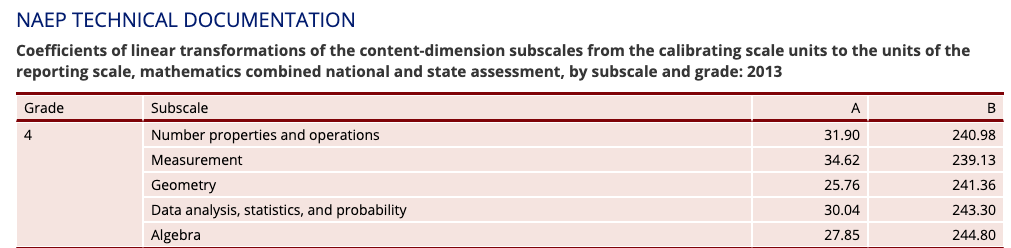
\includegraphics[width=0.7\linewidth]{images/5b_theta_to_scale_table}

\}

\textbackslash caption\{\url{https://nces.ed.gov/nationsreportcard/tdw/analysis/2013/trans_constants_math2013.aspx\%7D/label\%7Bfig:unnamed-chunk-11}\}
\textbackslash end\{figure\}

We provide an alternative theta\_to\_scale\_score function below, which
can weight these subscale parameters either by default proportions or by
their proportions in your selected test items, to most accurately mimic
NAEP scoring.

\begin{Shaded}
\begin{Highlighting}[]
\CommentTok{# Import table of transformation constants}
\NormalTok{scale_scores_raw <-}\StringTok{ }\KeywordTok{read.csv}\NormalTok{(}\StringTok{"Scale_Score_Equations.csv"}\NormalTok{)  }
  
\CommentTok{# Takes theta(s), returns scale score(s)}
\NormalTok{theta_to_scale_score <-}\StringTok{ }\ControlFlowTok{function}\NormalTok{(theta, }\DataTypeTok{weights =} \KeywordTok{c}\NormalTok{(}\FloatTok{0.4}\NormalTok{, }\FloatTok{0.2}\NormalTok{, }\FloatTok{0.15}\NormalTok{, }\FloatTok{0.1}\NormalTok{, }\FloatTok{0.15}\NormalTok{))}
\NormalTok{\{}
  \CommentTok{# Complex version: weighted average of each of the five subscale equations}
  \CommentTok{# Default weights taken from here for 2013 grade 4 Math: }
  \CommentTok{# https://nces.ed.gov/nationsreportcard/tdw/analysis/scaling_determination_composite.aspx}
  \CommentTok{# Alternatively, user can provide weights customized to the actual distribution of questions used}
\NormalTok{  A =}\StringTok{ }\KeywordTok{weighted.mean}\NormalTok{(}\DataTypeTok{x =}\NormalTok{ scale_scores_raw}\OperatorTok{$}\NormalTok{A, }\DataTypeTok{w =}\NormalTok{ weights)}
\NormalTok{  B =}\StringTok{ }\KeywordTok{weighted.mean}\NormalTok{(}\DataTypeTok{x =}\NormalTok{ scale_scores_raw}\OperatorTok{$}\NormalTok{B, }\DataTypeTok{w =}\NormalTok{ weights)}
  \KeywordTok{return}\NormalTok{(}\DataTypeTok{scale_score =}\NormalTok{ A}\OperatorTok{*}\NormalTok{theta }\OperatorTok{+}\StringTok{ }\NormalTok{B)}
\NormalTok{\}}
\end{Highlighting}
\end{Shaded}

\hypertarget{appendix-5-creating-an-item-map-using-released-item-parameters-1}{%
\section{Appendix 5: Creating an item map, using released item
parameters}\label{appendix-5-creating-an-item-map-using-released-item-parameters-1}}

An item map takes test questions and pegs them to specific scale scores,
such that users can visualize which items a student of a given scale
score is likely have already mastered, and which items they are less
likely to answer correctly yet.

Example item map:
\url{https://www.nationsreportcard.gov/itemmaps/?subj=MAT\&grade=4\&year=2013}

NAEP says this about their item maps:

``NOTE: CR denotes a constructed-response question. SR denotes a
selected-response question. MC denotes a multiple-choice question.
Apparent differences between estimates may not be statistically
significant. Results are not shown for data points where the sample
sizes are insufficient to permit reliable estimates or where data are
not available. The position of a question on the scale represents the
scale score attained by students who had a 65 percent probability of
obtaining credit at a specific level of CR questions or polytomously
scored SR questions, a 74 percent probability of correctly answering a
four-option multiple-choice question, or a 72 percent probability of
correctly answering a five-option multiple-choice question in certain
subjects.''

In this section, we provide simple code to create item maps for any set
of items for which item difficulties are known

\begin{Shaded}
\begin{Highlighting}[]
\CommentTok{# Combine the table containing question descriptors (selected_items) with the table of item parameters (item_parameters)}
\NormalTok{combined_table <-}\StringTok{ }\KeywordTok{inner_join}\NormalTok{(selected_items, item_parameters, }\DataTypeTok{by =} \StringTok{"NAEP.ID"}\NormalTok{, }\DataTypeTok{copy =} \OtherTok{FALSE}\NormalTok{)}

\CommentTok{# This function takes item parameter(s) and a response probability and returns theta(s)}
\NormalTok{ip_and_RP_to_theta <-}\StringTok{ }\ControlFlowTok{function}\NormalTok{(data, }\DataTypeTok{RP =} \FloatTok{0.73}\NormalTok{)}
\NormalTok{\{}
  \CommentTok{# RP = response probability ("a student with scale score x should have a RP% chance of answering this item correctly")}
  \CommentTok{# RP defaults to 73% here, as NAEP uses RP = 74 for MC items with four choices, and RP = 72 for those with five options. }
  \CommentTok{# We split the difference here}
\NormalTok{  theta =}\StringTok{ }\NormalTok{data}\OperatorTok{$}\NormalTok{bj }\OperatorTok{-}\StringTok{ }\DecValTok{1}\OperatorTok{/}\NormalTok{\{D}\OperatorTok{*}\NormalTok{data}\OperatorTok{$}\NormalTok{aj\}}\OperatorTok{*}\KeywordTok{log}\NormalTok{((}\DecValTok{1} \OperatorTok{-}\StringTok{ }\NormalTok{RP)}\OperatorTok{/}\NormalTok{(RP }\OperatorTok{-}\StringTok{ }\NormalTok{data}\OperatorTok{$}\NormalTok{cj))}
  \KeywordTok{return}\NormalTok{(theta)}
\NormalTok{\}}

\NormalTok{combined_table}\OperatorTok{$}\NormalTok{map_theta <-}\StringTok{ }\KeywordTok{ip_and_RP_to_theta}\NormalTok{(}\DataTypeTok{data =}\NormalTok{ combined_table)}

\CommentTok{# Convert to scale score, round to 0dp}
\NormalTok{combined_table}\OperatorTok{$}\NormalTok{Scale_Score <-}\StringTok{ }\KeywordTok{round}\NormalTok{(}\KeywordTok{theta_to_scale_score}\NormalTok{(}\DataTypeTok{theta =}\NormalTok{ combined_table}\OperatorTok{$}\NormalTok{map_theta), }\DecValTok{0}\NormalTok{)}

\CommentTok{# Sort by map_theta}
\NormalTok{combined_table <-}\StringTok{ }\NormalTok{combined_table[}\KeywordTok{order}\NormalTok{(combined_table}\OperatorTok{$}\NormalTok{map_theta, }\DataTypeTok{decreasing =} \OtherTok{TRUE}\NormalTok{), ]}

\CommentTok{# Export out, in format similar to NAEP}
\KeywordTok{write.csv}\NormalTok{(combined_table[ , }\KeywordTok{colnames}\NormalTok{(combined_table) }\OperatorTok\StringTok{ }\KeywordTok{c}\NormalTok{(}\StringTok{"Subscale"}\NormalTok{, }\StringTok{"Scale_Score"}\NormalTok{, }\StringTok{"Description"}\NormalTok{)], }
          \DataTypeTok{file =} \StringTok{"Generated_Item_Map.csv"}\NormalTok{, }\DataTypeTok{row.names =}\NormalTok{ F)}
\end{Highlighting}
\end{Shaded}

\end{document}
